%% BMC Bioinformatics -- Research Article
%% Target journal: BMC Bioinformatics (Springer Nature / BioMed Central).
%% Section layout follows BMC Research Article format:
%%   Background, Results, Discussion, Conclusions, Methods, Declarations.
%% Compile: pdflatex main.tex  (twice, for refs)

\documentclass[11pt,a4paper]{article}

\usepackage[margin=1in]{geometry}
\usepackage{lineno}
\usepackage{amsmath}
\usepackage{graphicx}
\usepackage{booktabs}
\usepackage{array}
\usepackage{tabularx}
\usepackage{url}
\usepackage{xcolor}
\usepackage{authblk}
\usepackage[authoryear,round]{natbib}
\usepackage{tikz}
\usetikzlibrary{shapes.geometric, arrows.meta, positioning, fit}
\usepackage{hyperref}
\hypersetup{colorlinks=true,linkcolor=blue,citecolor=blue,urlcolor=blue}
\newcommand{\doi}[1]{\href{https://doi.org/#1}{\texttt{doi:#1}}}
\setlength{\emergencystretch}{1em}

\title{A direct-merge pipeline with matrix-completion imputation
  for integrative analysis of heterogeneous microarray gene
  expression datasets}

\author[1]{Author One\thanks{Lead contact: author.one@example.org}}
\author[1]{Author Two}
\author[1]{Author Three}
\affil[1]{Institute of Molecular Biology and Genetics,
  National Academy of Sciences of Ukraine, Kyiv, Ukraine}

\date{}

\begin{document}

\maketitle

\begin{abstract}
\noindent\textbf{Background:}
Integrative re-analysis of public microarray gene expression
datasets is limited by the fact that different array generations
target different subsets of the human gene catalog. Naive
intersection of gene lists across platforms discards informative
signal, while mean-imputation strategies can fabricate
biologically implausible values. A method is needed that recovers
cross-platform genes without compromising downstream differential
expression analysis.

\noindent\textbf{Results:}
We present a reproducible R pipeline that
(i)~loads probe-collapsed, ENTREZID-keyed expression matrices
from an arbitrary set of GEO studies;
(ii)~selects the minimum number of datasets in which a gene must
be present, either fixed by the user or auto-selected to keep the
fraction of missing values below a configurable cap;
(iii)~imputes the remaining missing entries with
\textit{softImpute} nuclear-norm matrix completion;
(iv)~applies reference-batch ComBat correction on the merged,
completed matrix; and
(v)~runs \textit{limma} differential expression with hard masking
of imputed cells, so that imputed values influence neither the
adjusted $p$-values nor the log-fold changes of the reported DEGs.
Applied to six placental/chorionic-villi datasets spanning four
microarray platforms from four vendors (Affymetrix, Illumina,
Applied Biosystems, and Agilent), the pipeline recovers $17{,}531$
testable genes from an intersection of only $8{,}260$, and
identifies $447$ differentially expressed genes
($|\text{logFC}| > 1$, FDR~$< 0.05$) between first- and
second-trimester placenta/chorionic villi.
Subsampling validation confirmed stable effect sizes across
sample compositions (Lin's CCC~$\ge 0.88$), and comparison with a
balanced two-dataset reference showed $91.5\%$ overlap of the
full-integration DEG list.

\noindent\textbf{Conclusions:}
Matrix-completion imputation enables integrative re-analysis of
heterogeneous microarray datasets without sacrificing gene
coverage. Hard masking of imputed cells in the differential
expression step ensures that all statistical calls are driven
exclusively by real measurements, while the imputed values serve
only to stabilise batch correction.
\end{abstract}

\noindent\textbf{Keywords:} microarray integration; matrix
completion; softImpute; ComBat; limma; placenta; chorionic villi;
differential expression.

\vspace{1em}
\linenumbers

%% =========================================================================
\section{Background}
%% =========================================================================

Meta-analysis of public transcriptomic datasets is a
cost-effective way to increase statistical power for subtle
biological contrasts and to cross-validate findings across
laboratories. The classical obstacle is batch effect: studies
generated on different dates, with different sample processing,
or with different array generations exhibit systematic technical
variation that overshadows biology unless corrected. Methods
such as ComBat
\citep{Johnson2007} and the broader \textit{sva} framework
\citep{Leek2012} address this problem when the datasets share
the same feature space.

A second, less-discussed obstacle is \emph{coverage
heterogeneity}: different microarray platforms print probes for
different subsets of the human gene catalog, and the
intersection shrinks rapidly as the number of platforms grows
(Table~\ref{tab:platforms}).
Historically, investigators have dealt with this either by
restricting the merged matrix to the \emph{inner join}
(intersection --- only genes measured on every platform are
kept, and the rest are discarded) or by taking an \emph{outer
join} (union --- every gene measured on at least one platform
is kept) and filling the resulting missing entries with
batch-specific gene means, a simple but naive imputation
strategy that introduces artificial structure resembling
biological signal. Neither option respects the low-rank
correlation structure of biological gene expression data ---
i.e.\ the fact that the expression of thousands of genes is
governed by a much smaller number of underlying regulatory
programmes, so that the full matrix can be well approximated
by a product of fewer latent factors.

This study extends a line of prior work by our group on
integrative analysis of placental/chorionic-villi microarray data. An earlier
methods paper \citep{Lykhenko2021a} established the consecutive
ComBat-based integration strategy used here as a baseline,
and a companion application paper \citep{Lykhenko2021b}
characterised differential gene expression across the three
physiological trimesters of pregnancy using the
intersection-only variant of that pipeline. The present
study addresses the principal limitation of those earlier
analyses --- loss of several thousand genes at the
cross-platform intersection step --- by replacing intersection
with auditable matrix-completion imputation.

The sole reason imputation is needed in this pipeline is that
ComBat requires a complete matrix: it cannot estimate batch
parameters from a matrix with structural holes. The quality of
the imputed values therefore matters not for the downstream
differential expression test --- \textit{limma} does not need a
complete matrix and in our pipeline never sees the imputed cells
(they are hard-masked to weight zero) --- but for ComBat itself,
whose batch-effect estimates will be distorted if the filled
values are poor. Here we describe a
\emph{direct-merge} workflow that implements this strategy ---
\textit{softImpute} \citep{Mazumder2010,Hastie2015}, a nuclear-norm
regularised low-rank matrix completion method, fills structural
holes so that ComBat operates on a full-rank matrix, after which imputed cells are effectively
removed from \textit{limma} differential expression analysis.
We apply this method to the first vs.~second trimester contrast
(1\_2) in placental/chorionic-villi gene expression, reporting gene coverage,
imputation accuracy, differential expression counts, and
subsampling validation of result stability.

%% =========================================================================
\section{Results}
%% =========================================================================

\subsection{Gene recovery and missingness}
\label{sec:recovery}

For the 1\_2 comparison (6 datasets, 117 samples) with
the minimum dataset-presence threshold set to $k = 1$ (every gene present in at least one dataset), the
merged matrix grows from 8{,}260 genes (intersection, $k = 6$)
to 17{,}531 genes, with the missing-cell fraction rising to
29.4\%. Gene recovery and missingness for each threshold $k$ are
shown in Table~\ref{tab:recovery}.

\begin{table}[h]
\centering
\footnotesize
\begin{tabular}{@{}rrrr@{}}
\toprule
\textbf{min\_datasets ($k$)} & \textbf{Genes retained} &
  \textbf{Missing cells} & \textbf{\% missing} \\
\midrule
$\ge$6/6 &  8{,}260 &         0 &  0.0\,\% \\
$\ge$5/6 & 11{,}239 &  90{,}084 &  6.9\,\% \\
$\ge$4/6 & 13{,}617 & 248{,}619 & 15.6\,\% \\
$\ge$3/6 & 17{,}223 & 587{,}410 & 29.2\,\% \\
$\ge$2/6 & 17{,}387 & 593{,}398 & 29.2\,\% \\
$\ge$1/6 & 17{,}531 & 603{,}190 & 29.4\,\% \\
\bottomrule
\end{tabular}
\caption{Gene recovery and resulting missingness for each
  minimum dataset-presence threshold $k$, 1\_2 comparison
  (6 datasets, First Trimester vs.~Second Trimester,
  117 samples). At $k = 6$ (intersection only), 8{,}260 genes
  are retained with zero imputation. At $k = 1$ (any gene in
  $\ge$1 dataset), 17{,}531 genes are retained after the
  per-group safety drop, with
  29.4\% of cells requiring imputation.}
\label{tab:recovery}
\end{table}

The per-group imputation safety check
removed 298 genes that were absent from every
Second-Trimester sample (Table~\ref{tab:coverage}). Of the
9{,}569 genes needing imputation in $\ge\!1$ dataset, 9{,}271
had at least one real measurement in \emph{both} groups and were
retained.

\begin{table}[h]
\centering
\footnotesize
\begin{tabular}{@{}lr@{}}
\toprule
\textbf{Gene category (1\_2 comparison)} & \textbf{Count} \\
\midrule
Genes present in all 6 datasets (no imputation needed) & 8{,}260 \\
Genes needing imputation in $\ge$1 dataset            & 9{,}569 \\
\quad with $\ge$1 real value in BOTH groups (kept)    & 9{,}271 \\
\quad missing entirely from Second Trimester (dropped) & 298 \\
\quad missing entirely from First Trimester (dropped)  & 0 \\
\midrule
Final merged matrix size                               & 17{,}531 \\
\bottomrule
\end{tabular}
\caption{Per-group imputation safety audit for the 1\_2
  comparison. The final merged matrix contains 8{,}260 fully
  observed genes plus 9{,}271 partially observed genes that
  passed the both-groups-have-evidence rule.}
\label{tab:coverage}
\end{table}

The block-structured missingness pattern is shown in
Figure~\ref{fig:staircase}.

\begin{figure}[htbp]
\centering
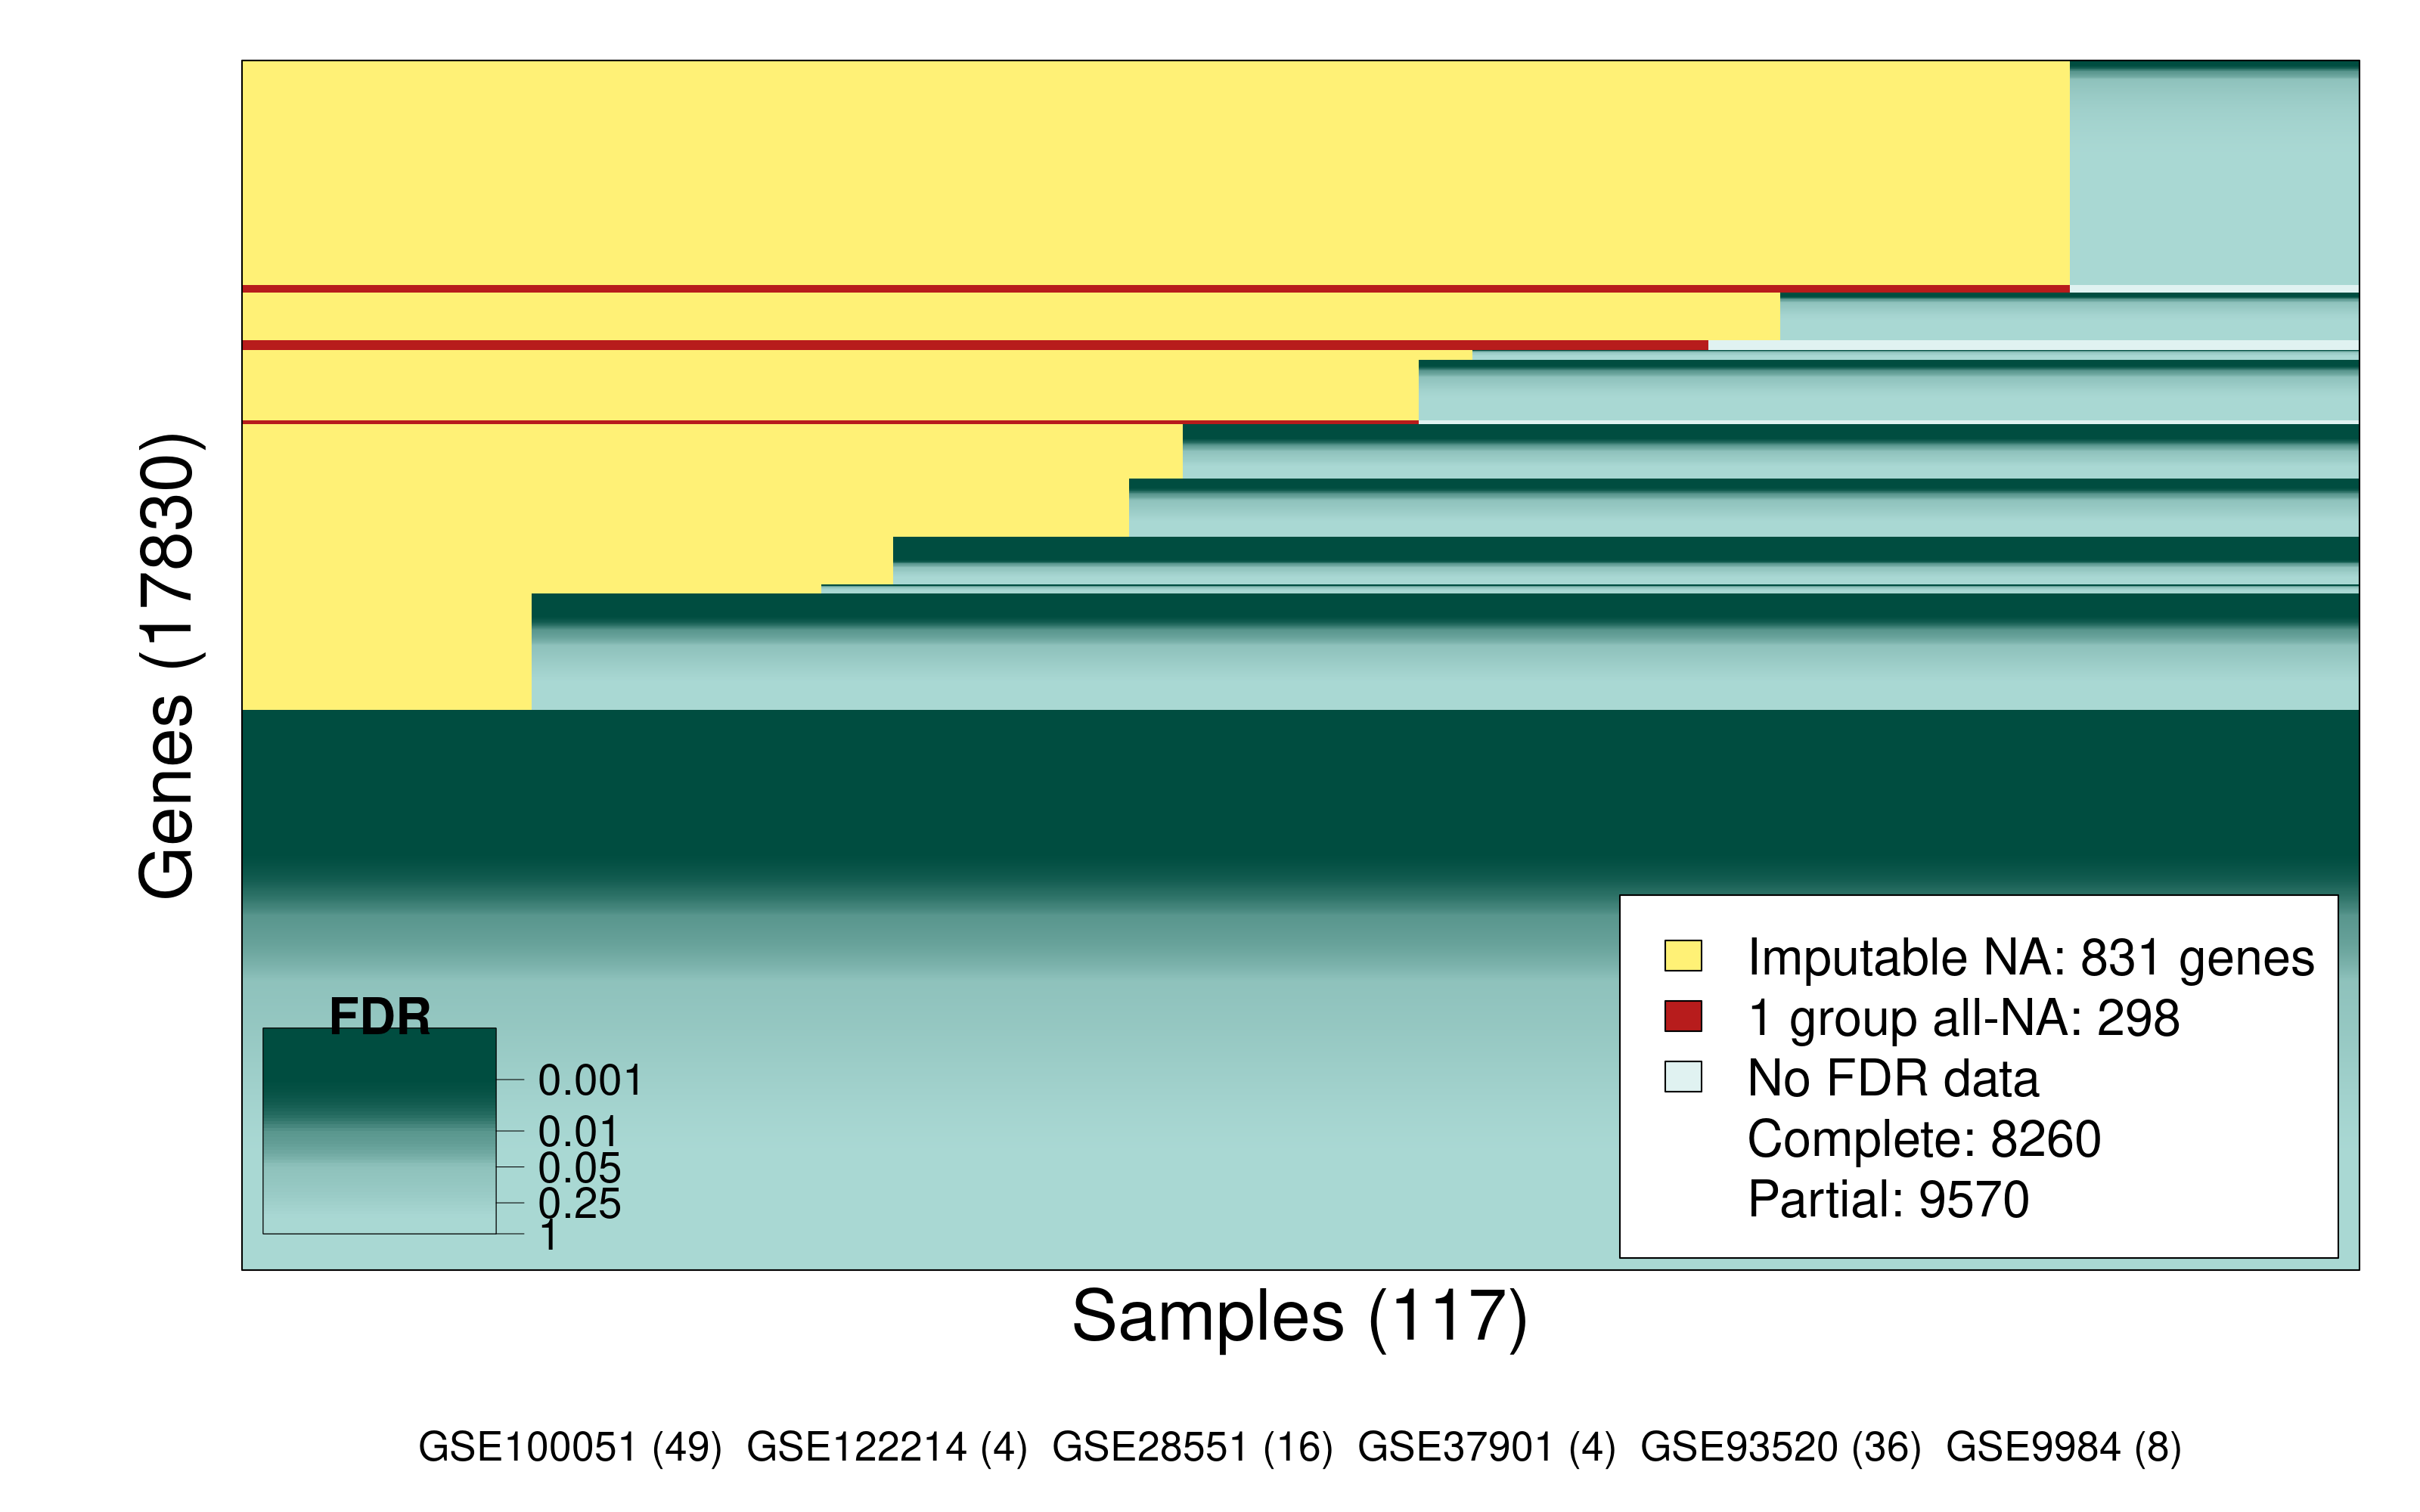
\includegraphics[width=\textwidth]{figures/fig_na_staircase.png}
\caption{Block-structured missingness in the merged
  gene-by-sample matrix (17{,}829 protein-coding genes $\times$
  117 samples, sorted by dataset). Each column is a sample;
  each row is a gene. Yellow cells are missing (\texttt{NA}):
  the gene is not targeted by that sample's microarray platform.
  Blue shading shows FDR values from the softImpute $+$
  ComBat-ref differential expression result (darker = more
  significant). The red band marks the 298 genes missing
  entirely from the second-trimester group (dropped by the
  per-group safety rule). Without
  imputation, only the bottom block (8{,}260 genes present in
  all six datasets, no yellow) is usable --- the entire upper
  portion of the matrix (9{,}569 genes) would be discarded by
  an inner-join merge, despite containing well-measured,
  biologically informative signal in the majority of datasets.
  Note that many genes in the imputed region (upper block)
  show significant FDR values (dark blue), confirming that
  the discarded genes carry real differential expression signal
  that an intersection-only analysis would miss.}
\label{fig:staircase}
\end{figure}

\subsection{Imputation accuracy}
\label{sec:imputation}

Imputation accuracy was quantified by leave-out cross-validation:
a random 10\% of the observed entries were masked, imputed, and
compared against ground truth. Three independent repetitions
were run; each repeat used a freshly drawn mask. Three metrics are
reported for each repeat:
\begin{itemize}
  \item \emph{Pearson $r$} --- correlation between imputed and
    true values across the held-out cells; a unit-free measure
    of how well the method ranks high- and low-expression cells
    relative to each other. $r = 1$ is perfect, $r = 0$ is
    chance.
  \item \emph{RMSE} (root-mean-square error) ---
    $\sqrt{\frac{1}{n}\sum_{ij}(\hat x_{ij} - x_{ij})^2}$, the
    square root of the mean squared imputation error. Because
    the per-dataset expression matrices entering the pipeline
    are already log$_2$-transformed, RMSE is in units of
    $\log_2$ expression, so an RMSE of $0.33$ corresponds to a
    typical imputation error of $\approx 2^{0.33}\!\approx\!1.26\times$
    (a 27\% fold-change relative to the true value). RMSE
    penalises large errors more heavily than small ones because
    of the squaring.
  \item \emph{MAE} (mean absolute error) ---
    $\frac{1}{n}\sum_{ij}|\hat x_{ij} - x_{ij}|$, the mean of
    the per-cell absolute errors. Also in $\log_2$ units, but
    unlike RMSE it treats every error linearly and is therefore
    more robust to a handful of poorly-imputed outlier cells.
\end{itemize}
Results are given in Table~\ref{tab:imputation}.
Under random-cell masking (the classical in-distribution
leave-out), \textit{softImpute} achieved a mean Pearson
correlation of $r = 0.994$ with ground truth (RMSE $= 0.330$;
MAE $= 0.220$). Under the more stringent gene--dataset block
masking, which simulates the real missingness pattern, accuracy
dropped to $r = 0.816$ (RMSE $= 1.52$; MAE $= 1.17$). The
block-mask result is the more informative benchmark: it tests
the imputer's ability to reconstruct an entire gene's expression
profile in a dataset where that gene was never measured ---
exactly the scenario that arises in cross-platform merging.

\begin{table}[h]
\centering
\footnotesize
\begin{tabular}{@{}llrrrr@{}}
\toprule
\textbf{Mask type} & \textbf{Method} &
  \textbf{Cells masked} & \textbf{Pearson $r$} &
  \textbf{RMSE} & \textbf{MAE} \\
  & & \textbf{per rep} & & & \\
\midrule
random cells        & softImpute & 154{,}948 &
  $0.994 \pm 0.000$ & $0.330 \pm 0.001$ &
  $0.220 \pm 0.000$ \\
\addlinespace
gene--dataset block & softImpute & 144{,}811 &
  $0.816 \pm 0.002$ & $1.523 \pm 0.010$ &
  $1.165 \pm 0.006$ \\
\bottomrule
\end{tabular}
\caption{Leave-out cross-validation of \textit{softImpute}
  imputation accuracy (1\_2 comparison, 6 datasets, 17{,}531
  genes). Each row shows the mean $\pm$ standard deviation over
  three independent repeats. Two masking strategies are reported:
  \emph{random cells} draws individual observed cells uniformly
  at random; \emph{gene--dataset block} masks every cell for a
  randomly chosen (gene, dataset) pair, simulating the real
  missingness pattern where a gene is entirely absent from one
  dataset. Block masking is a substantially harder test because
  the imputer must reconstruct an entire gene's profile in a
  dataset with no direct observations. For block-mask validation,
  the gene--dataset pair pool is restricted to genes fully
  observed across all six datasets (so masking removes one dataset's worth of
  observations from an otherwise complete row); partially observed
  genes are excluded because masking them would leave rows too
  sparse for \texttt{biScale} to converge.}
\label{tab:imputation}
\end{table}

\subsection{Batch correction}

Figure~\ref{fig:pca} shows PCA projections of the
batch-corrected expression matrices. In both cases --- the
intersection-only matrix (8{,}260 genes) and the
\textit{softImpute}-completed matrix (17{,}531 genes) ---
ComBat-ref removes the dominant batch effect: samples separate
primarily by trimester (PC1) rather than by dataset. The
imputed matrix preserves this separation while doubling the
gene space.

\begin{figure}[htbp]
\centering
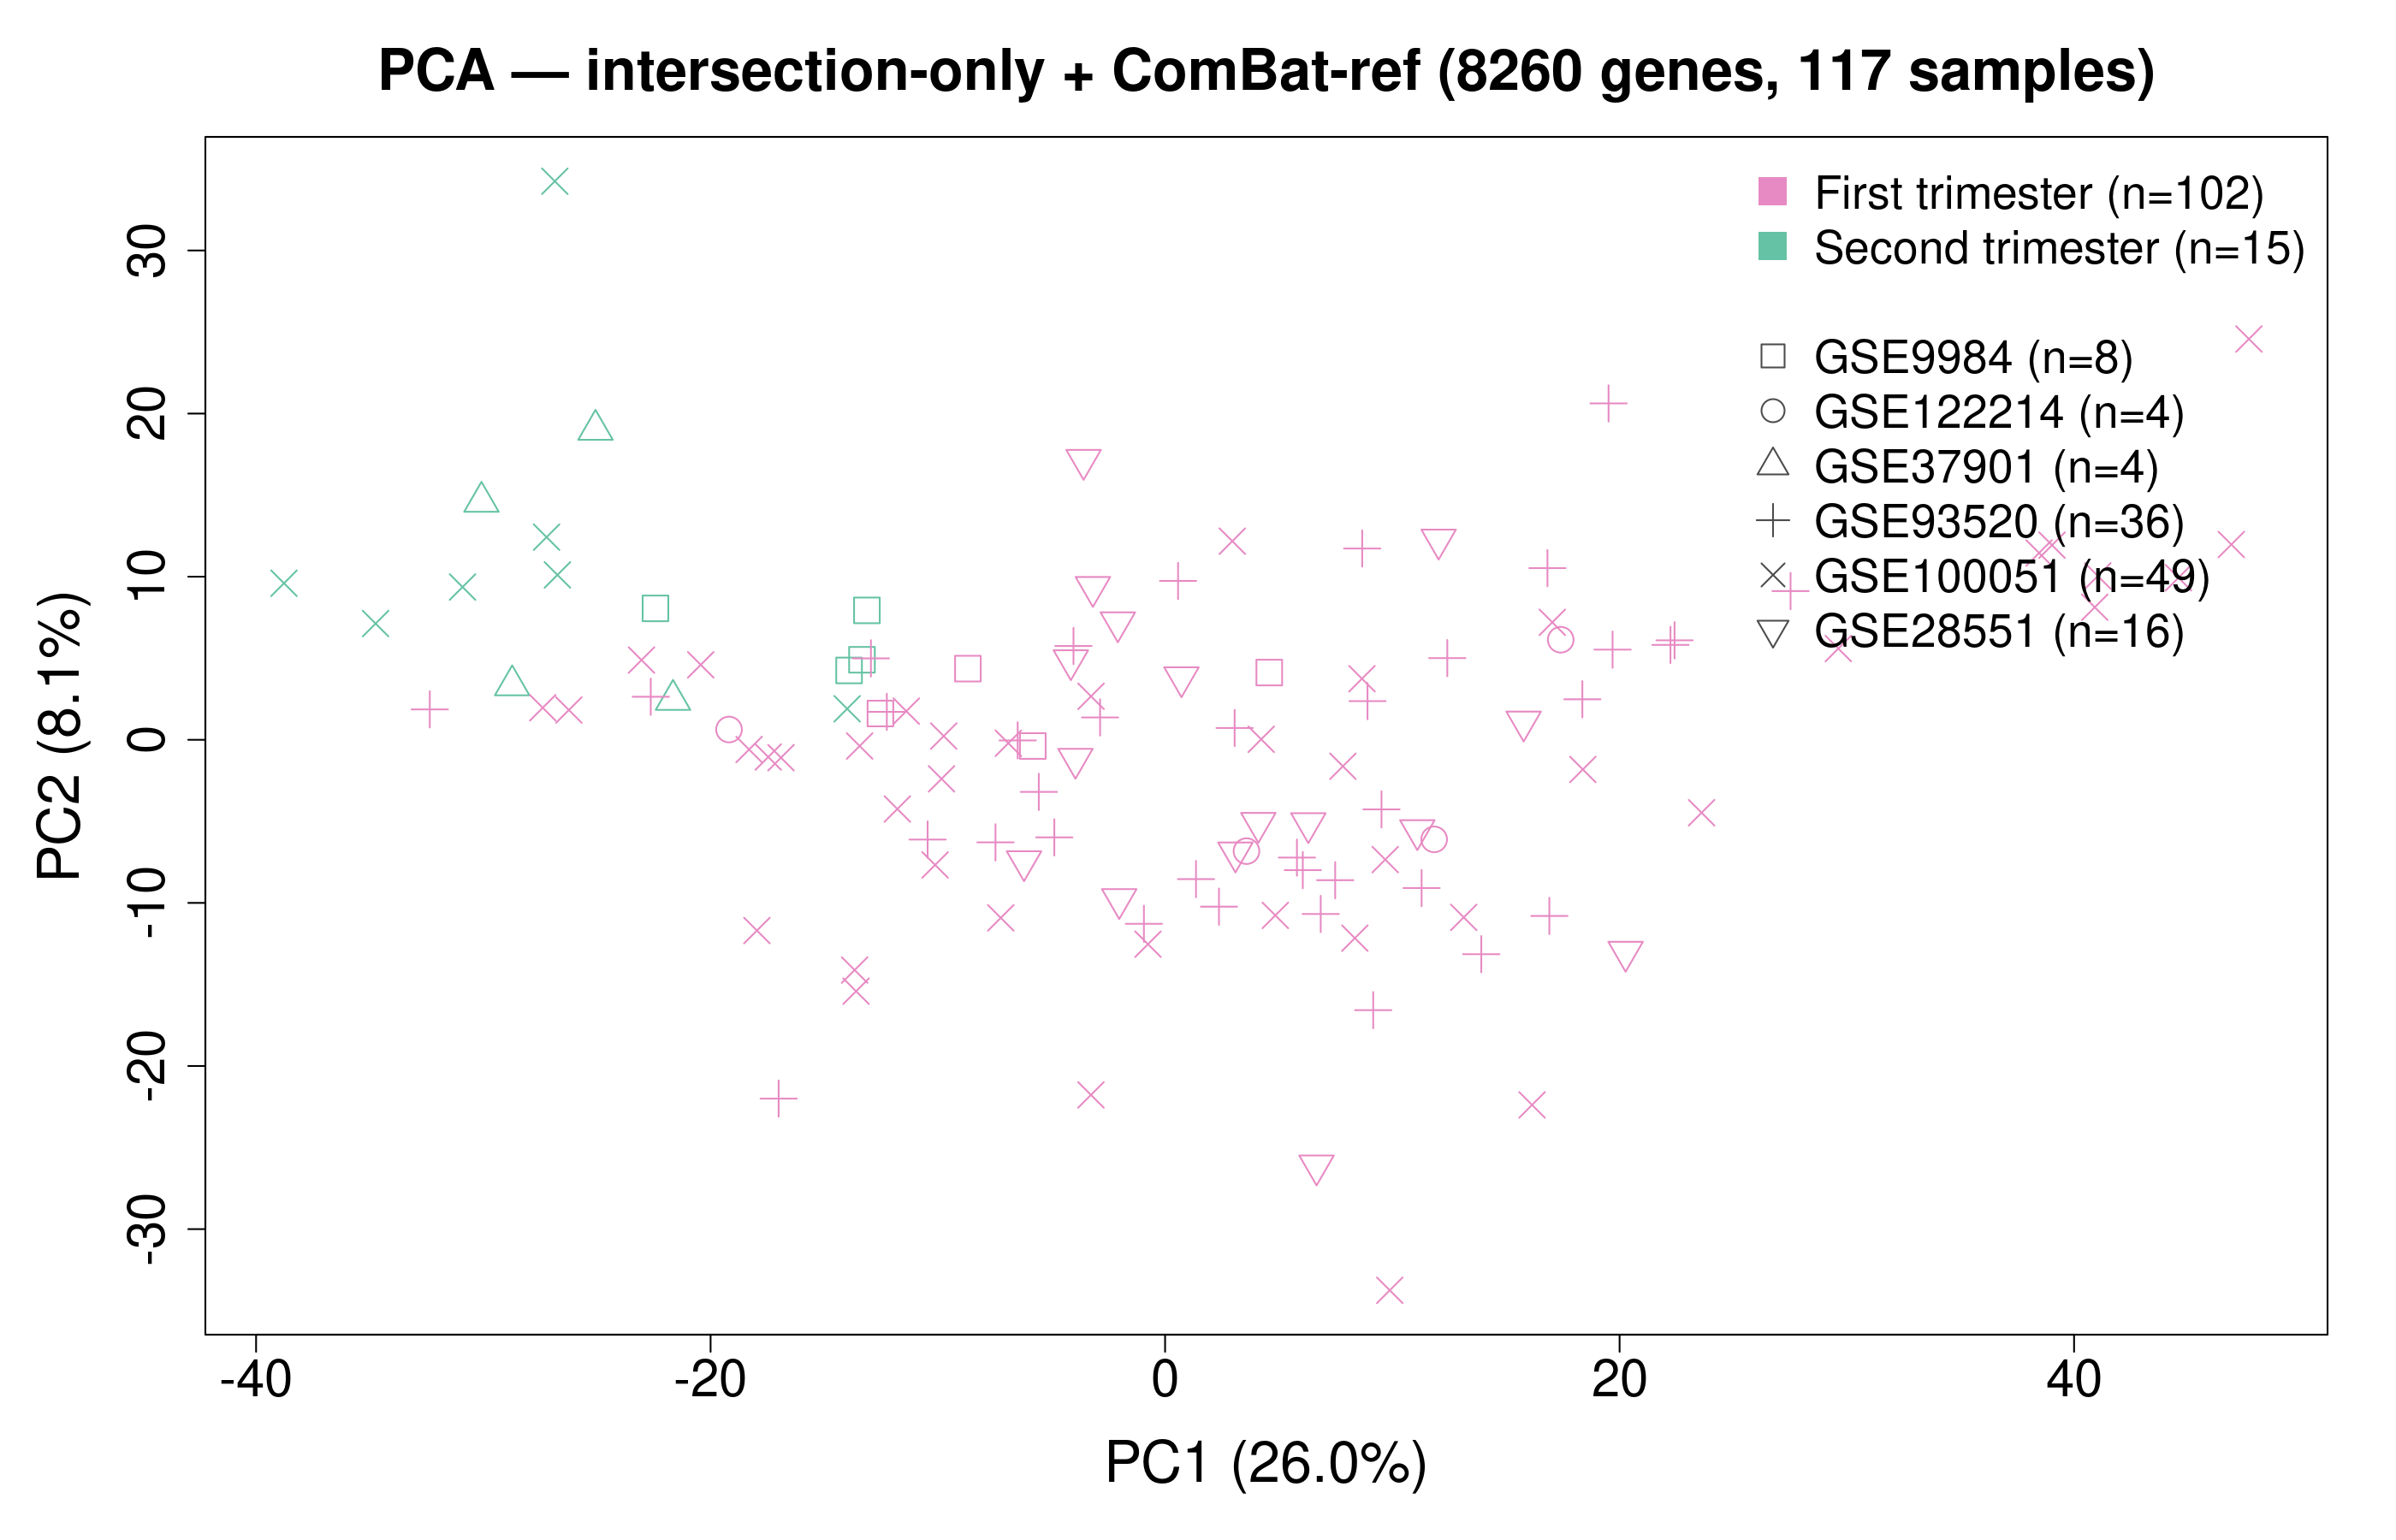
\includegraphics[width=0.49\textwidth]{figures/fig_pca_intersection.png}
\hfill
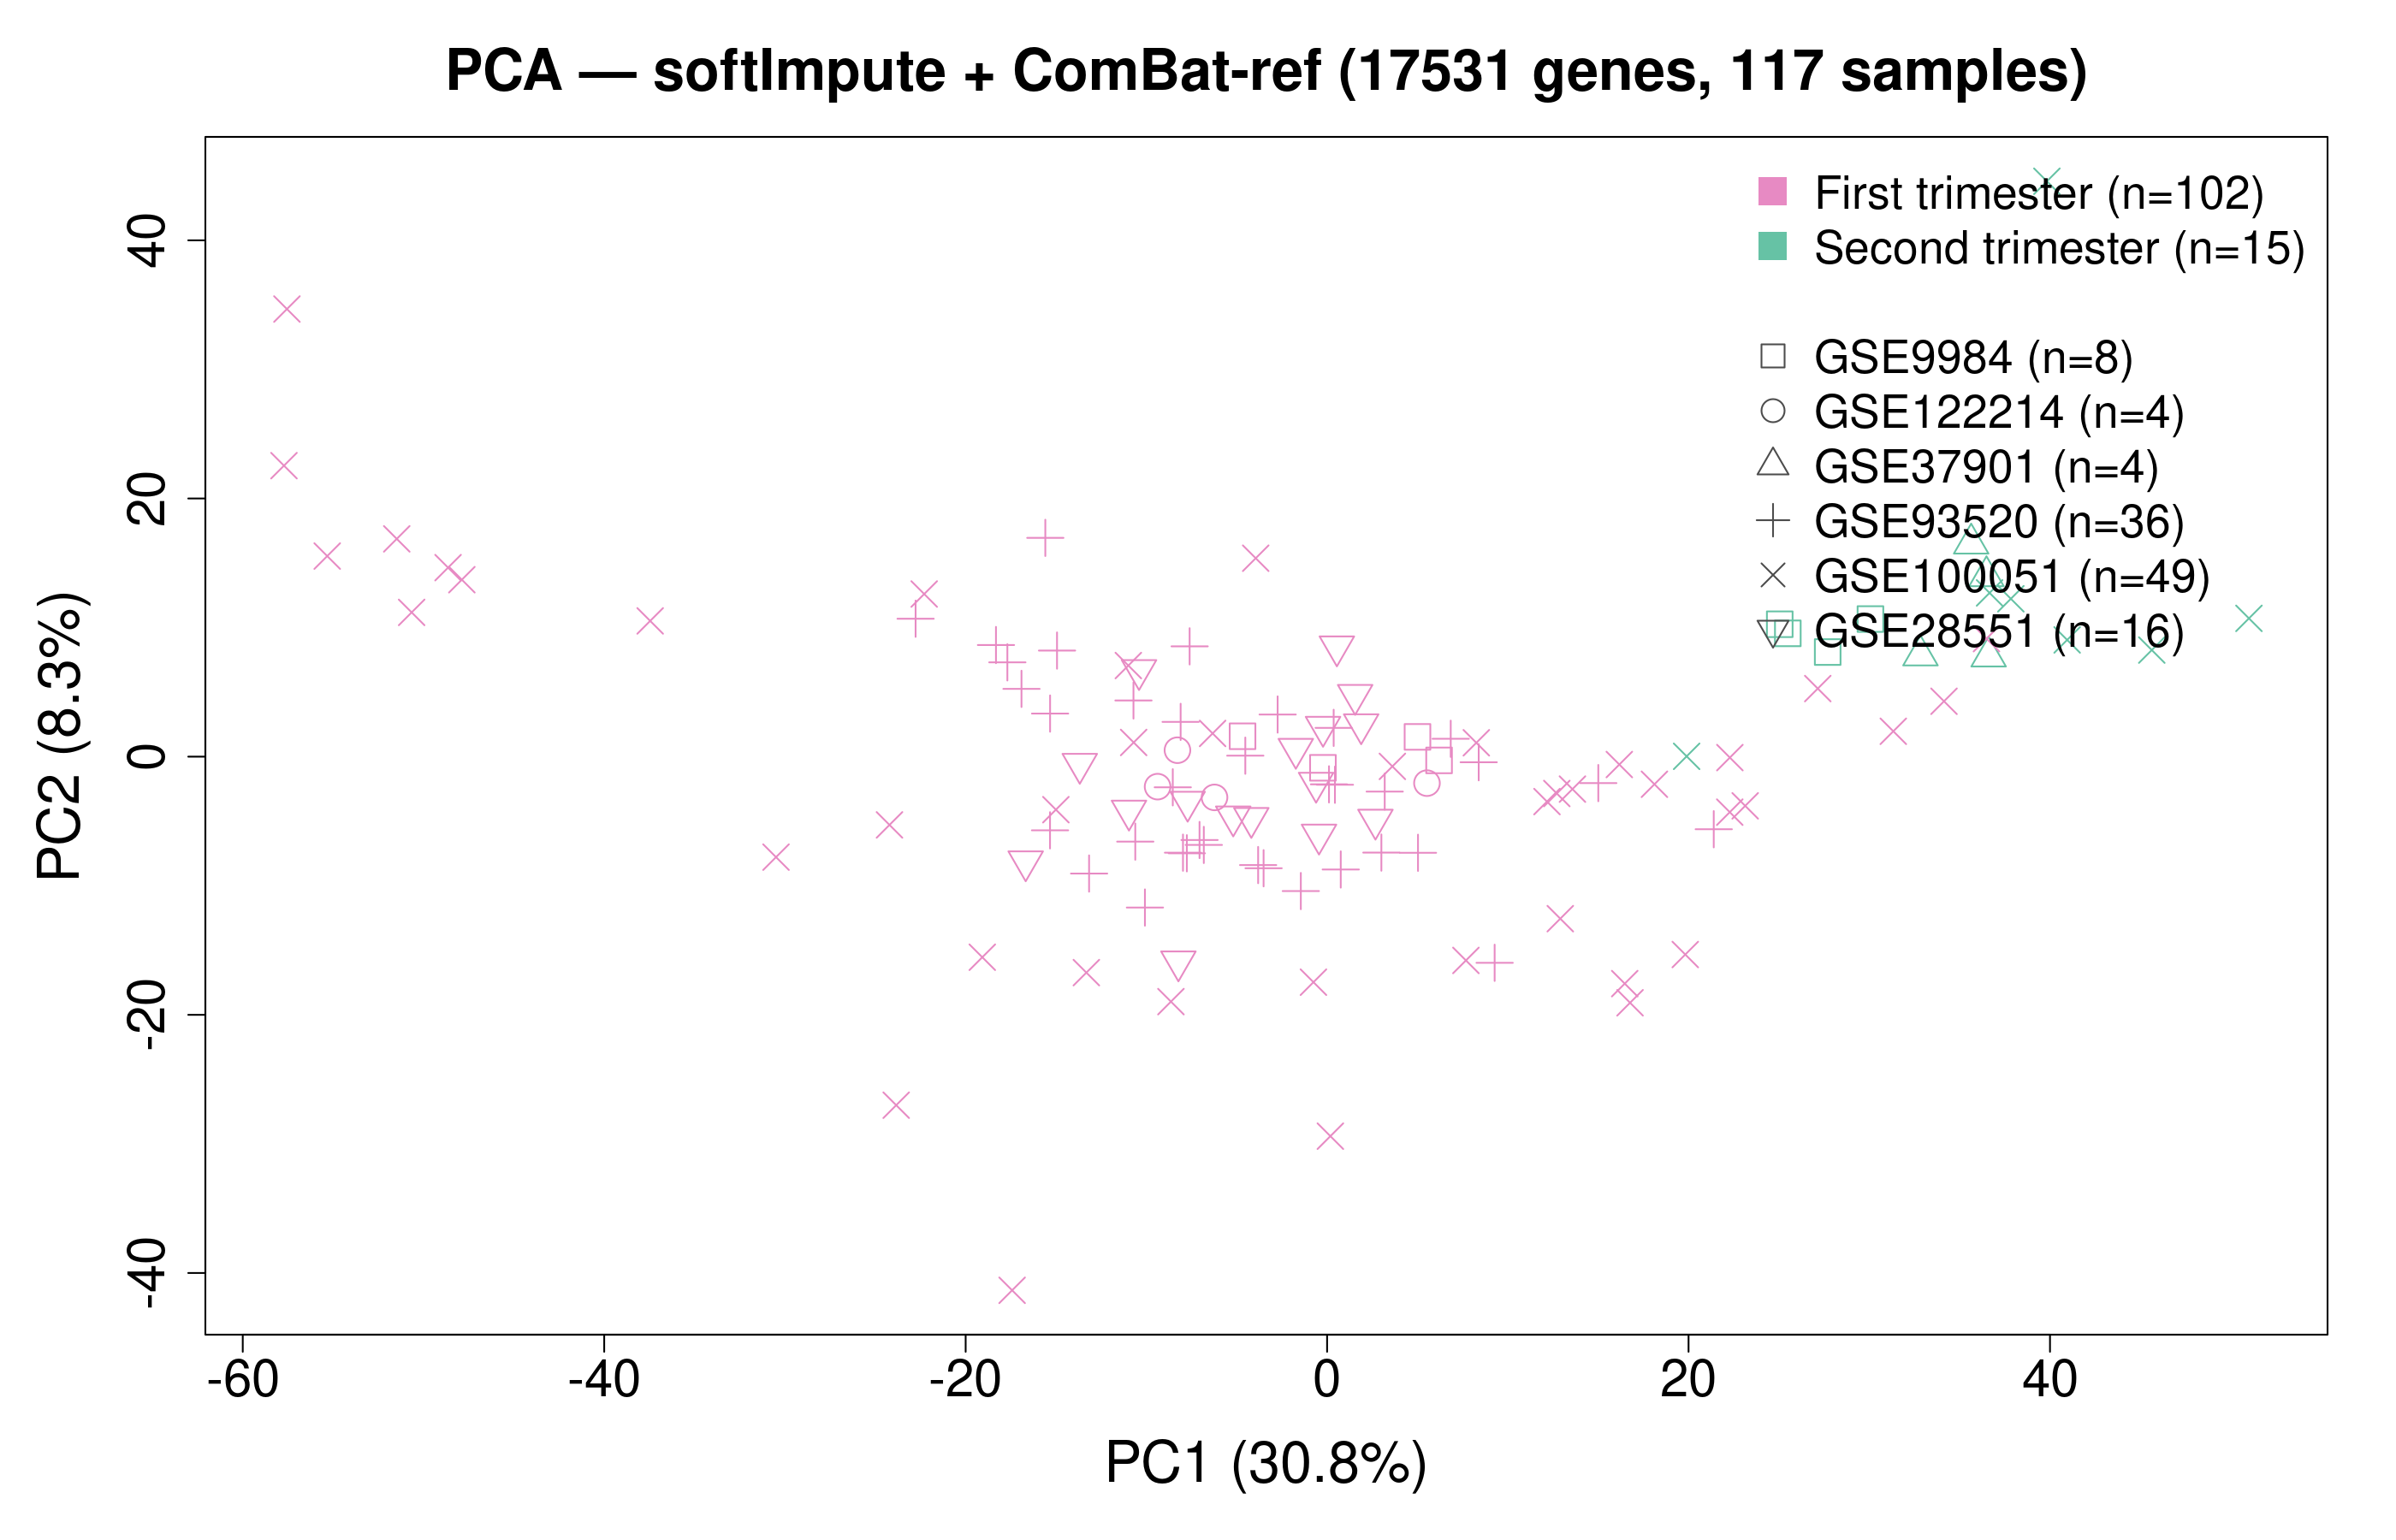
\includegraphics[width=0.49\textwidth]{figures/fig_pca_softimpute.png}
\caption{PCA of batch-corrected expression matrices after
  reference-batch ComBat (ref = GSE100051). \textbf{Left:}
  intersection-only (8{,}260 genes, no imputation).
  \textbf{Right:} \textit{softImpute}-completed (17{,}531
  genes). Colour indicates trimester (blue = first, vermillion =
  second); shape indicates dataset. In both panels, PC1
  separates the two trimesters, confirming that ComBat-ref
  removes batch effects without collapsing the biological
  contrast. The softImpute panel includes 9{,}271 additional
  genes recovered by imputation.}
\label{fig:pca}
\end{figure}

\subsection{Differential expression}
\label{sec:de}

Table~\ref{tab:de} reports the number of genes called
significant at $\text{adj.P.Val} < 0.05$ and
$|\text{logFC}| > 1$ across four method combinations, together
with the earlier result from \citet{Lykhenko2021a} for
comparison. The intersection of all six datasets collapses
to only 8{,}260 common genes, but enabling \textit{softImpute}
recovers 17{,}531 testable genes. With reference-batch ComBat
(ComBat-ref) correction, this lifts the DEG count from 221
(intersection only) to 447 (softImpute), adding 226 newly
called genes (195 up, 31 down).

Importantly, imputation does not distort the effect-size
estimates of genes that were already measurable without it.
For the 8{,}260 genes shared between the intersection-only and
\textit{softImpute} analyses, the log fold-change correlation
is near-perfect (Pearson $r = 0.998$), with a median absolute
difference of $0.014$ $\log_2$ units and $99\%$ of genes
differing by less than $0.09$. The additional genes recovered
by imputation therefore expand the testable feature space
without altering the differential expression landscape of the
originally observed genes.

The earlier intersection-only analysis by
\citet{Lykhenko2021a}, which was restricted to four
Affymetrix-only datasets (GSE122214, GSE22490, GSE37901,
GSE9984; 13~first-trimester $+$ 9~second-trimester $=$
22~samples), reported 327 DEGs with $|\text{logFC}| > 1$ from
an intersection of 20{,}261 genes --- a larger feature space
than our six-dataset intersection (8{,}260) because all four
datasets share the same Affymetrix platform. The present
pipeline recovers comparable or larger DEG counts from a
more diverse, multi-vendor cohort, while more than quintupling
the sample size to 117.

\begin{table}[h]
\centering
\footnotesize
\begin{tabular}{@{}llcrrrr@{}}
\toprule
\textbf{Imputation} & \textbf{Normalisation} &
  \textbf{Datasets} & \textbf{$n$ genes} &
  \textbf{Significant} & \textbf{Up} & \textbf{Down} \\
\midrule
\multicolumn{7}{@{}l}{\textit{Lykhenko et al.\ 2021 (4 Affy datasets, 22 samples)}} \\[2pt]
none       & ComBat     & 4 & 20{,}261 & 327 & --- & --- \\
\midrule
\multicolumn{7}{@{}l}{\textit{This study (6 multi-vendor datasets, 117 samples)}} \\[2pt]
none       & ComBat     & 6 &  8{,}260 & 221 & 175 &  46 \\
none       & ComBat-ref & 6 &  8{,}260 & 221 & 174 &  47 \\
softImpute & ComBat     & 6 & 17{,}531 & 416 & 346 &  70 \\
softImpute & ComBat-ref & 6 & 17{,}531 & 447 & 369 &  78 \\
\bottomrule
\end{tabular}
\caption{Differential expression counts for the 1\_2 comparison
  (First Trimester vs.~Second Trimester). The top row shows the
  earlier result from \citet{Lykhenko2021a} using four
  same-platform Affymetrix datasets (22 samples, intersection
  only); per-direction counts were not reported. The bottom
  block shows the present study with six multi-vendor datasets
  (117 samples). ``none'' denotes intersection-only analysis (no
  imputation). ComBat-ref uses GSE100051 as the reference batch.
  Imputed-cell weight $w = 0$ (hard masking) for all softImpute
  runs. Thresholds: $\text{adj.P.Val} < 0.05$,
  $|\text{logFC}| > 1$.}
\label{tab:de}
\end{table}

\subsection{Subsampling validation}
\label{sec:validation}

To assess the robustness of the differential expression results
to sample composition, we performed a suite of subsampling
validation tests on the 1\_2 comparison (6 datasets, 102
first-trimester $+$ 15 second-trimester $=$ 117 healthy
placental/chorionic-villi samples; reference: 447~DEGs at FDR${}<0.05$,
$|\text{logFC}|>1$). All tests reused the reference run's
imputed matrix to eliminate \textit{softImpute} stochasticity and
isolate the effect of sample composition.

\paragraph{Test~1: first-trimester subsampling.}
All 15 second-trimester samples were retained and the
first-trimester pool was subsampled at sizes
$N \in \{10, 15, 20, 25, 30, 40, 50, 60, 80, 102\}$
(30~iterations per size). Three key findings emerged
(Figure~\ref{fig:convergence}):

\begin{enumerate}
  \item \textbf{Effect sizes are stable.} Lin's concordance
    correlation coefficient \citep{Lin1989}
    (CCC) between subsample and
    full-run log fold-changes exceeded $0.88$ even at
    $N\!=\!10$ and rose monotonically to $1.0$ at $N\!=\!102$
    (Figure~\ref{fig:ccc}). Unlike Pearson~$r$, which measures
    only the strength of the linear association, CCC also
    penalises systematic shifts in location or scale ---
    two vectors with $r = 1$ but different means or variances
    will have $\text{CCC} < 1$ --- making it a stricter test of
    numerical agreement between effect-size estimates.
  \item \textbf{DEG list overlap converges gradually.} Median
    Jaccard index against the full run rose from $0.54$ at
    $N\!=\!10$ to $1.0$ at $N\!=\!102$
    (Figure~\ref{fig:convergence}, left panel).
  \item \textbf{Retention of reference DEGs is high.}
    At $N\!=\!10$, subsamples retained a median of $90\%$ of
    the 447 reference DEGs, rising to $93\%$ at $N\!=\!30$
    (Figure~\ref{fig:retention}, first panel). The apparent
    Jaccard drop at small sizes is primarily driven by novel
    DEGs entering the subsample list (genes with noisy
    effect-size estimates that stochastically cross the
    $|\text{logFC}|\!>\!1$ threshold), not by loss of true
    positives.
\end{enumerate}

\paragraph{Comparison with a balanced independent reference.}
To test whether the design imbalance --- some datasets
contribute samples from only one trimester, which can bias
ComBat batch-effect estimates --- inflates the DEG
list, we compared against a balanced 2-dataset reference
(GSE100051 $+$ GSE9984; 46 first-trimester $+$ 11
second-trimester samples; regular ComBat; 416~DEGs). Of the
447 full-integration DEGs, $91.5\%$ ($409/447$) also appeared in
the balanced reference (Jaccard $= 0.901$). The integration
does not manufacture signal: $98.3\%$ ($409/416$) of the
balanced reference's DEGs are retained, and log fold-change agreement (CCC) exceeds
$0.99$ for the full pool (Figure~\ref{fig:ccc}, right panel).
Even at $N\!=\!10$, subsamples retained $\sim\!90\%$ of the
balanced reference DEGs (Figure~\ref{fig:retention}, second
panel).

\paragraph{FDR-only versus FDR$+$logFC thresholding.}
DEG lists defined by FDR alone ($\sim\!6{,}700$ genes) were
substantially less stable than those filtered by both FDR and
$|\text{logFC}|\!>\!1$ (median Jaccard $\sim\!0.5$ vs.\ $0.71$
at $N\!=\!30$; see Figure~\ref{fig:convergence}, right panel
vs.\ left panel). The $|\text{logFC}|$ threshold selects the
reproducible core of genes with large, consistent effect sizes.
FDR-only retention of the full-run gene set was also lower
($\sim\!51\%$ at $N\!=\!10$ vs.\ $90\%$ for FDR$+$logFC;
Figure~\ref{fig:retention}, third panel), confirming that
thousands of FDR-only genes are statistically significant but
have near-zero fold changes that are not reproducible across
subsamples.

\paragraph{Test~2: balanced subsampling.}
Equal numbers of samples ($n \in \{4, 8, 12, 15\}$) were drawn
from each trimester (30~iterations per size). Balanced
subsamples showed qualitatively similar convergence to
unbalanced ones (Figure~\ref{fig:convergence}, middle panel),
indicating that the design imbalance does not drive the observed
instability.

\paragraph{Test~3: stratified split-half.}
The full sample was randomly split into two halves maintaining
the trimester ratio (50~iterations). Median Jaccard between
halves was $0.40$, reflecting the limited statistical power
of 7--8 second-trimester samples per half. However, each half
retained a median of $84\%$ of the full-run DEGs
(Figure~\ref{fig:split_half}, bottom left), and log fold-change
CCC between halves was $0.70$ (Figure~\ref{fig:split_half}, top
right). FDR-only retention per half was much lower ($\sim\!51\%$;
Figure~\ref{fig:split_half}, bottom right), reinforcing the
value of the $|\text{logFC}|$ threshold. The split-half Jaccard
of $0.40$ is typical for microarray studies with small contrast
groups and does not indicate fragility of the core result.

\begin{figure}[htbp]
\centering
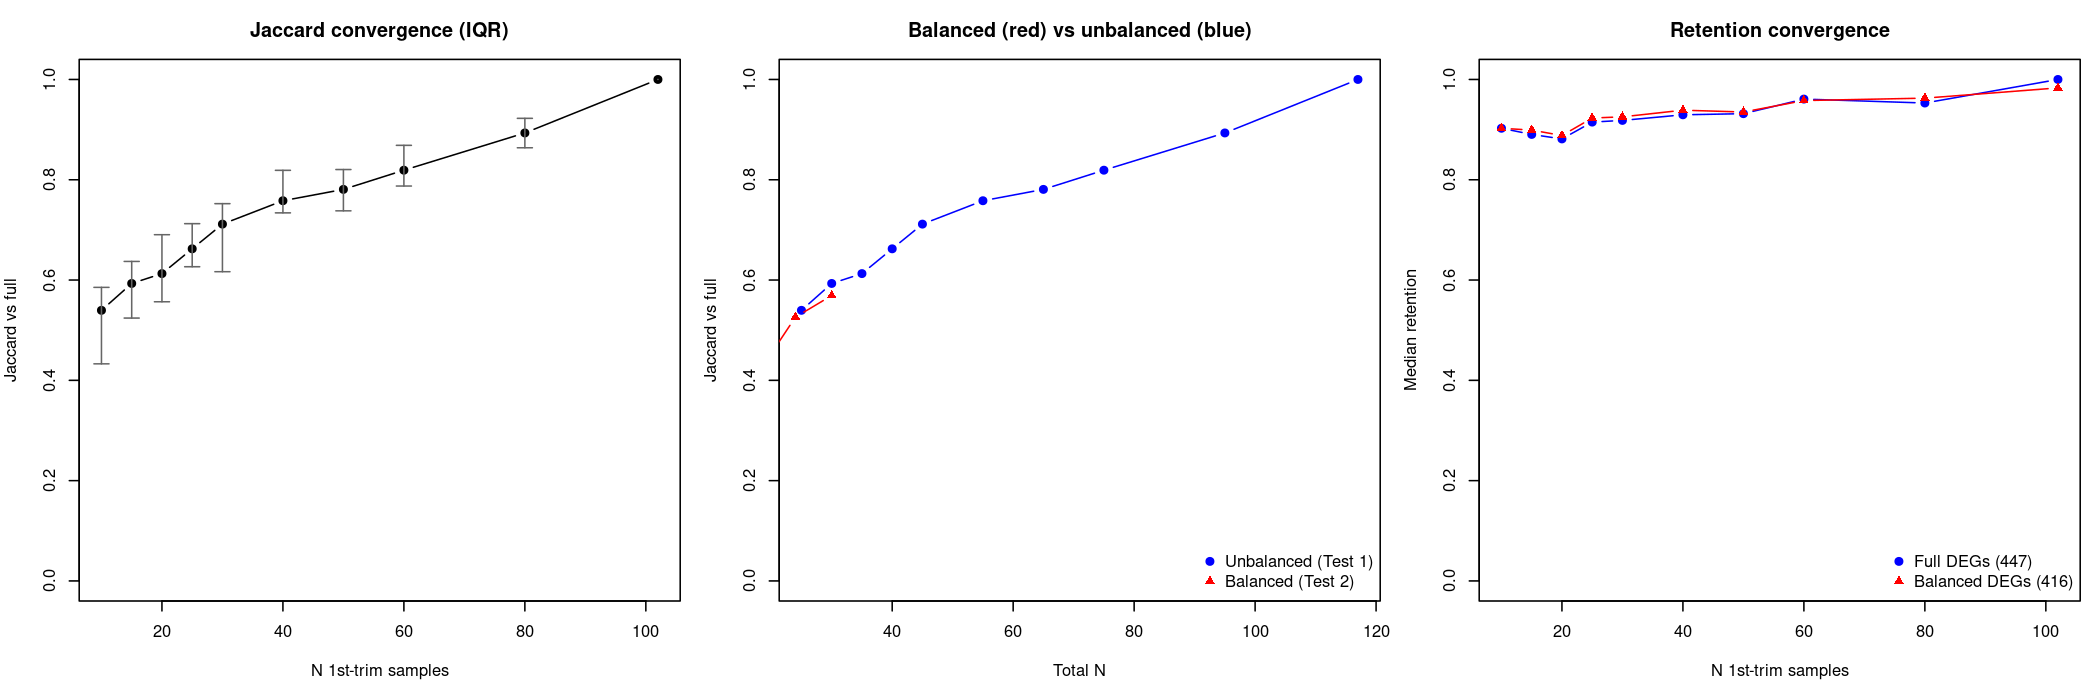
\includegraphics[width=\textwidth]{figures/fig_validation_convergence.png}
\caption{Subsampling validation summary. \textbf{Left:}
  Jaccard index of DEG lists versus the full-run reference
  as a function of first-trimester sample size (median with
  IQR). \textbf{Middle:} balanced (equal per trimester) vs.\
  unbalanced subsampling, both measured against the full run.
  \textbf{Right:} median retention of reference DEGs (blue:
  full integration, 447~DEGs; red: balanced 2-dataset
  reference, 416~DEGs) as a function of first-trimester
  sample size.}
\label{fig:convergence}
\end{figure}

\begin{figure}[htbp]
\centering
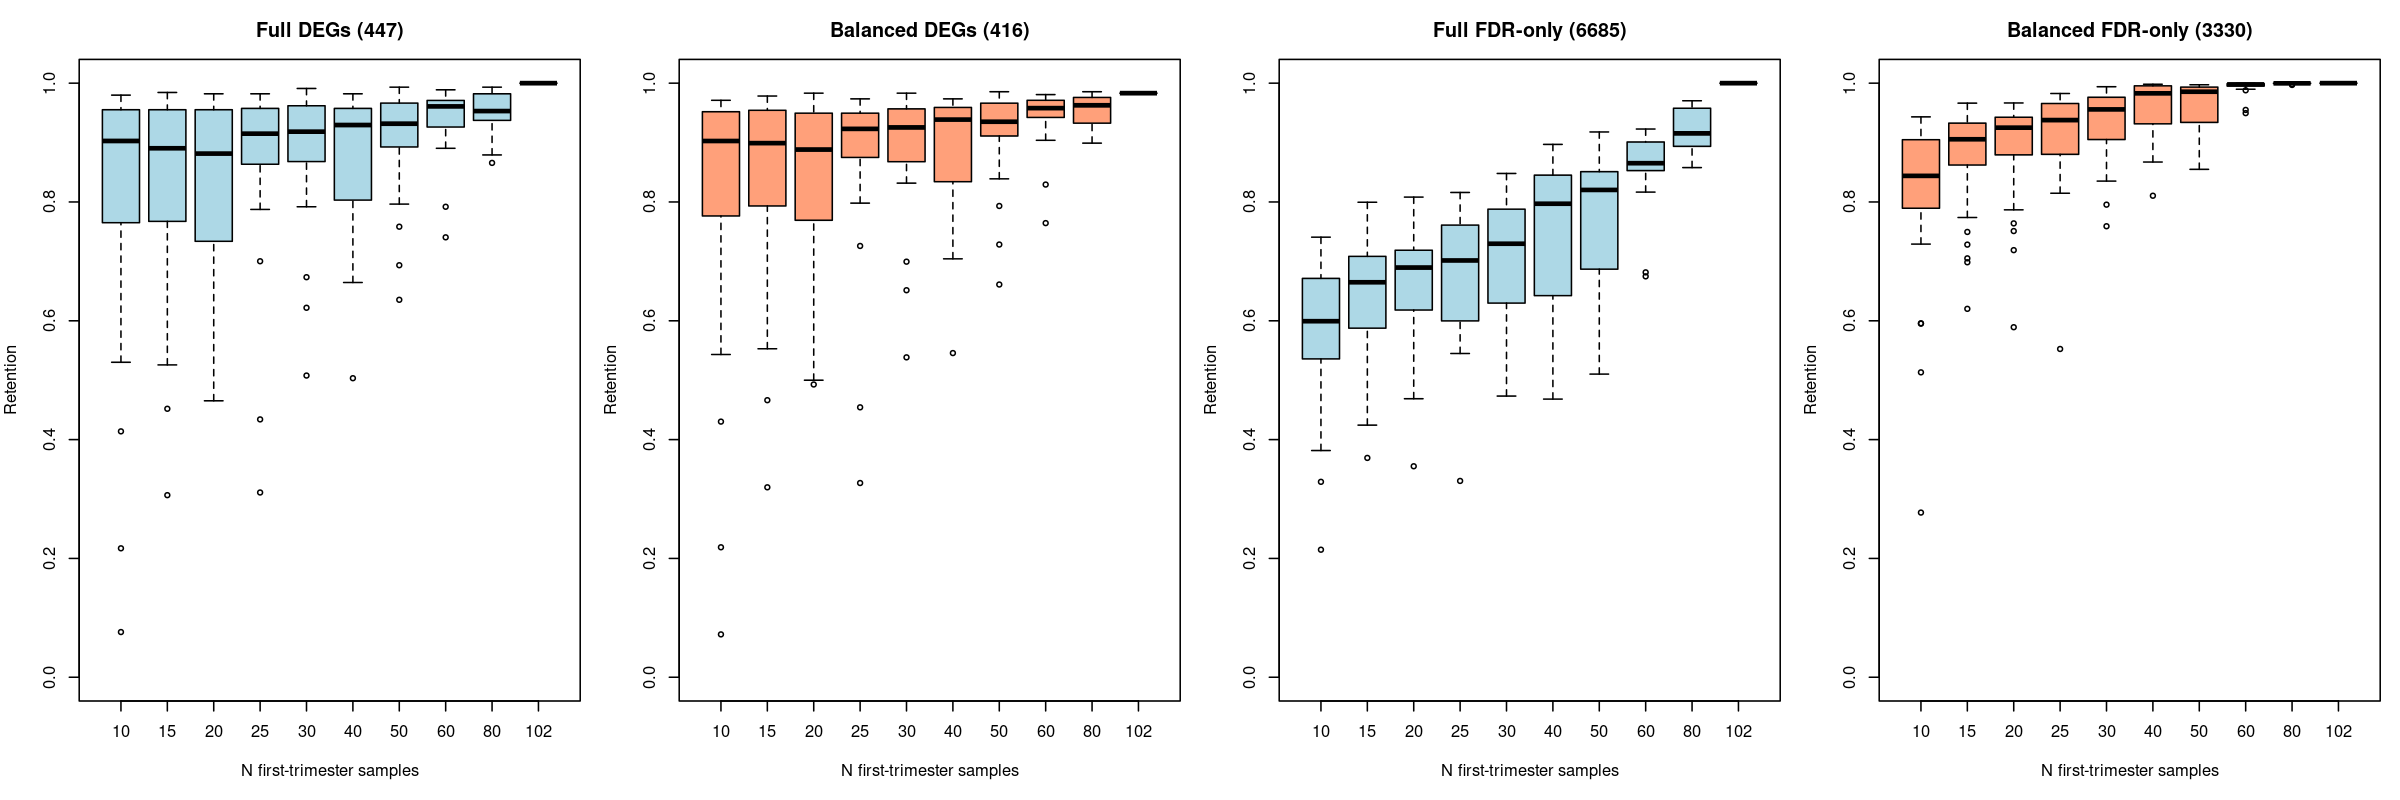
\includegraphics[width=\textwidth]{figures/fig_validation_retention.png}
\caption{Retention of reference DEGs across subsampling sizes.
  Each panel shows the fraction of a given reference set's DEGs
  that appear in the subsample's DEG list. From left to right:
  full-run DEGs (FDR$+$logFC, 447~genes); balanced-reference
  DEGs (FDR$+$logFC, 416~genes); full-run FDR-only DEGs
  (6{,}685~genes); balanced-reference FDR-only DEGs
  (3{,}330~genes).}
\label{fig:retention}
\end{figure}

\begin{figure}[htbp]
\centering
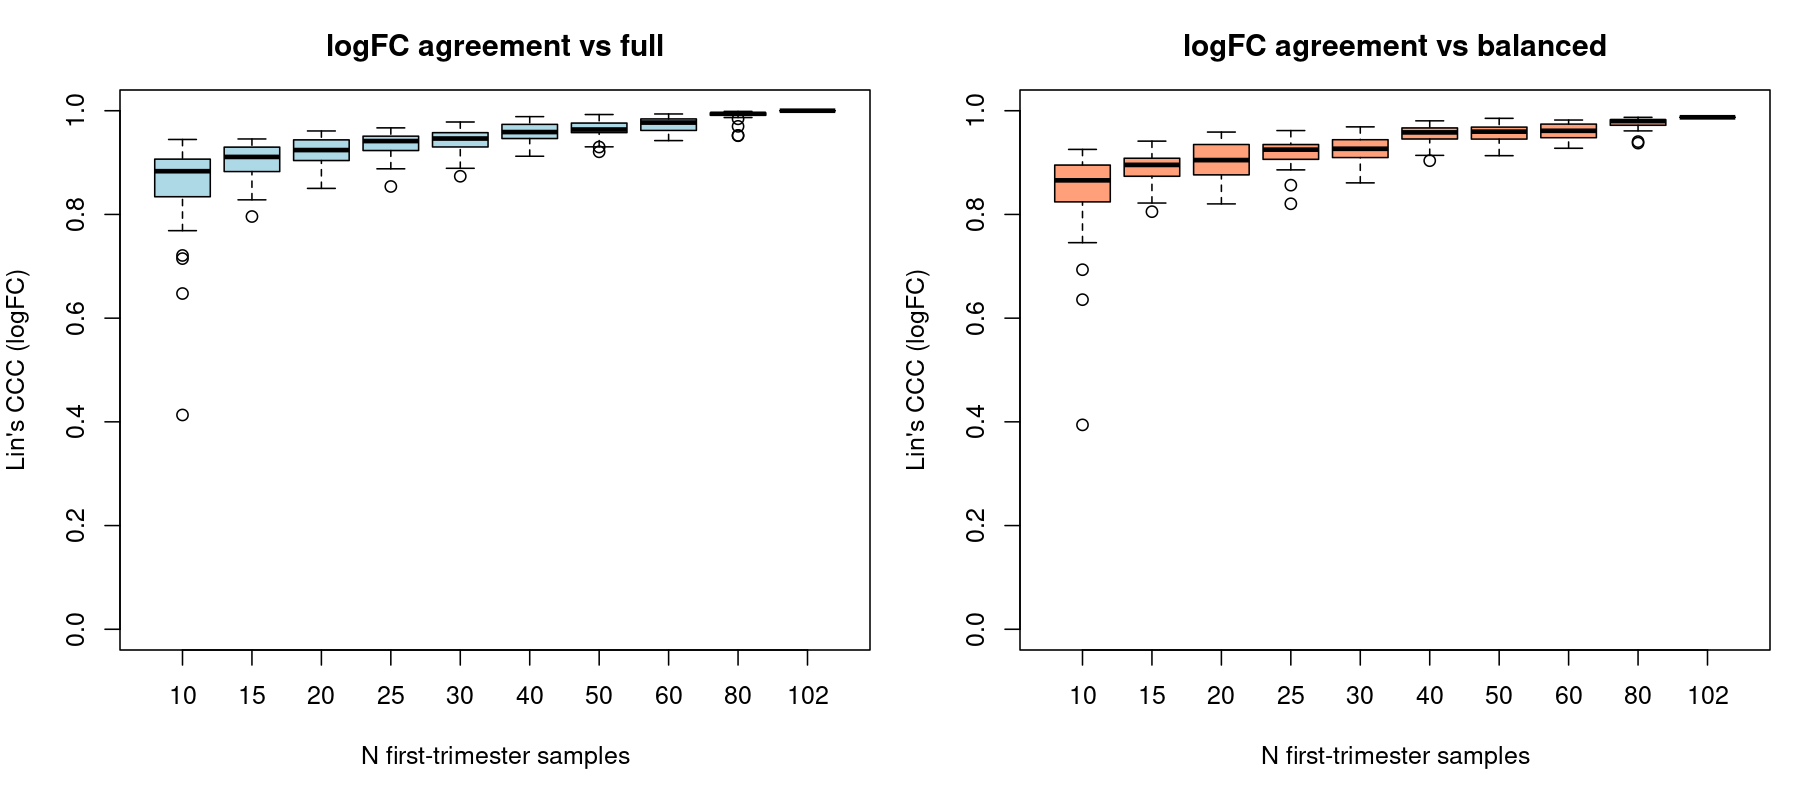
\includegraphics[width=\textwidth]{figures/fig_validation_ccc.png}
\caption{Log fold-change agreement (Lin's concordance
  correlation coefficient) between subsampled and reference
  runs. \textbf{Left:} versus the full 6-dataset integration.
  \textbf{Right:} versus the balanced 2-dataset reference.
  CCC~$= 1$ only when log fold-changes are numerically
  identical; unlike Pearson~$r$, it penalises systematic
  scaling or offset.}
\label{fig:ccc}
\end{figure}

\begin{figure}[htbp]
\centering
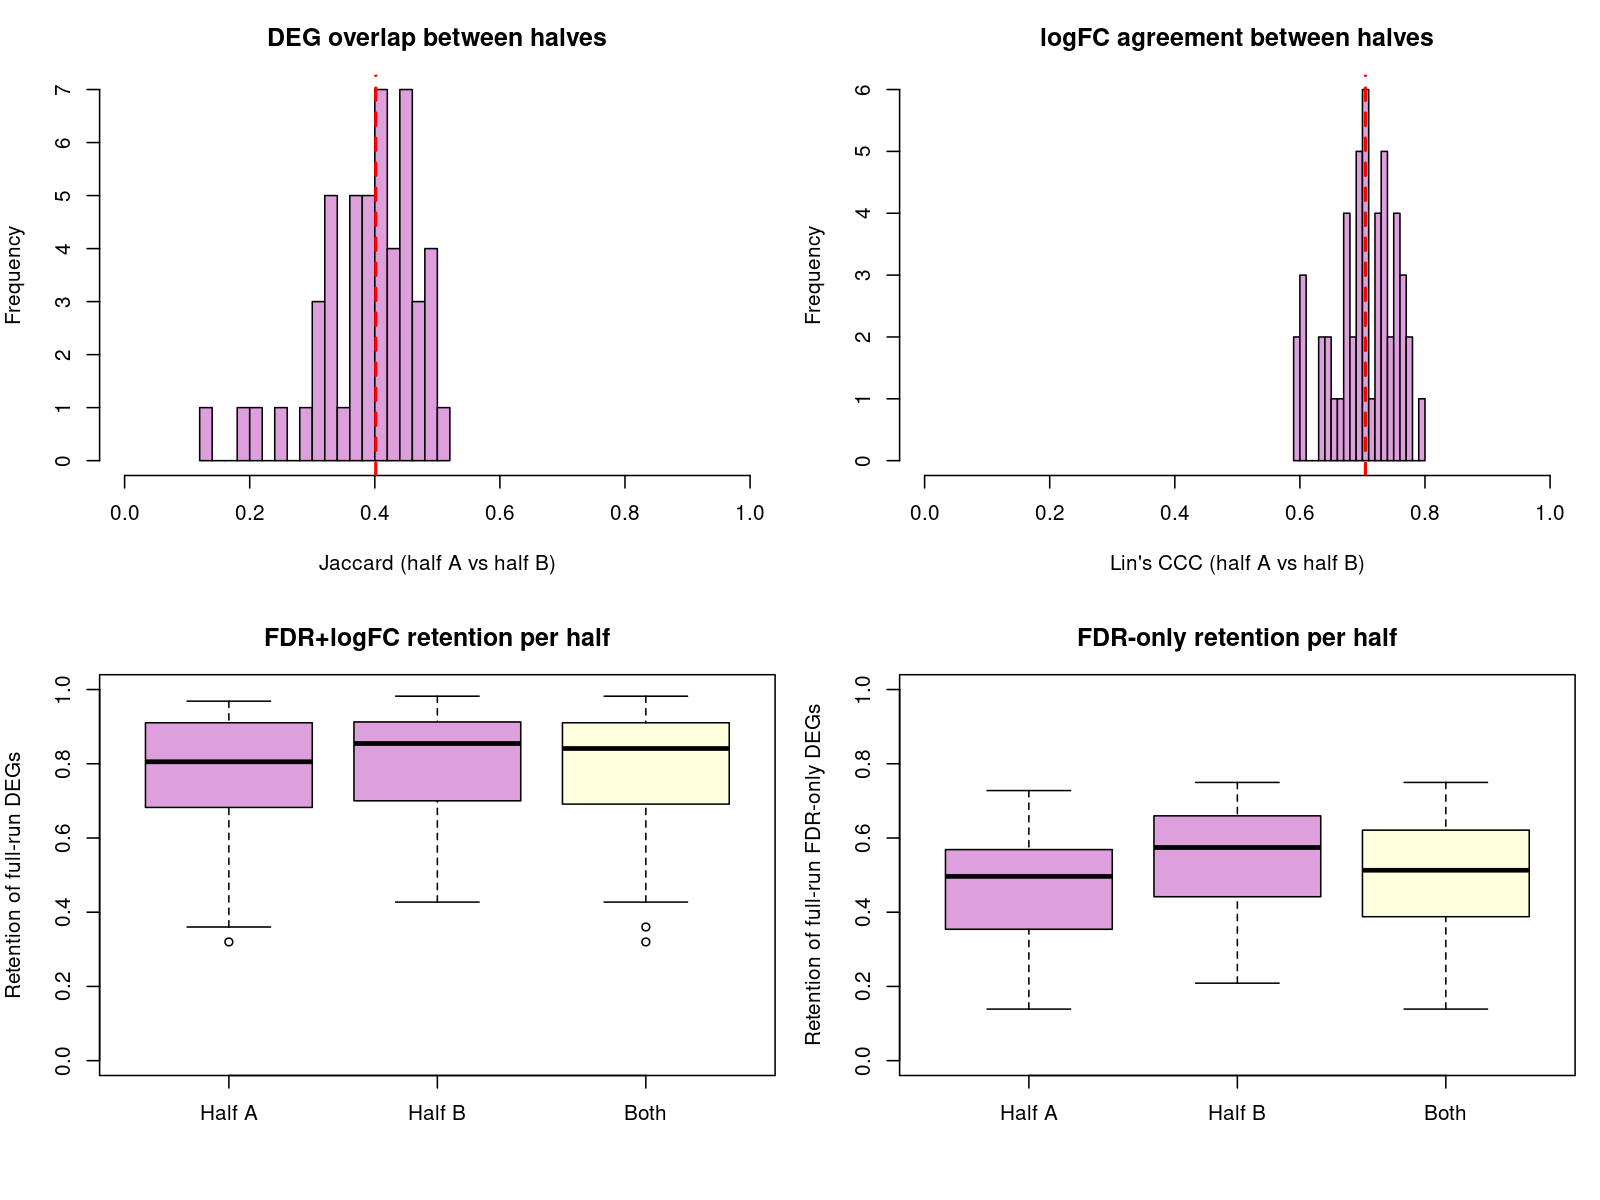
\includegraphics[width=\textwidth]{figures/fig_validation_split_half.png}
\caption{Stratified split-half validation (50~iterations).
  \textbf{Top left:} Jaccard between halves' DEG lists.
  \textbf{Top right:} Lin's CCC of log fold-changes between
  halves. \textbf{Bottom left:} retention of full-run DEGs
  (FDR$+$logFC) per half. \textbf{Bottom right:} retention of
  full-run FDR-only DEGs per half.}
\label{fig:split_half}
\end{figure}

%% =========================================================================
\section{Discussion}
%% =========================================================================

\subsection{Relation to prior work}

Imputing missing values in gene expression studies is not new,
but the specific setting of this paper --- filling
\emph{gene-by-dataset block holes} in a matrix produced by
merging several bulk microarray studies --- sits at the
intersection of two bodies of work that have so far developed
largely in parallel.

\paragraph{Within-study microarray imputation.}
The de-facto standard for recovering missing values in a single
microarray study is \texttt{KNNimpute}, introduced by
\citet{Troyanskaya2001} and reviewed extensively by
\citet{Aittokallio2010} and \citet{Liew2011}. These methods were
designed for the small fraction of cells (1--20\%) lost inside
one study to hybridisation failures, image noise, or bad spots.
The missingness is approximately at random at the cell level, and
KNN is well suited to it. None of these works address the
structurally different problem in which a whole gene is absent
from a whole dataset because the platform did not probe it.

\paragraph{Knowledge-assisted imputation.}
A separate line of work has augmented expression-based imputation
with external biological knowledge.
\citet{Tuikkala2006} replaced the purely expression-based distance
in KNN with a combined metric that incorporates Gene Ontology
semantic similarity, showing improved accuracy when the number of
experimental conditions is small.
\citet{Tuikkala2008} extended this idea to histone acetylation
data (HAIimpute), using chromatin modification profiles as an
additional source of gene similarity for neighbour selection.
Both approaches are designed for within-study cell-level
missingness and require auxiliary annotations (GO terms) or
matched epigenomic data (ChIP profiles) that may not be available
for all genes or studies in a cross-platform meta-analysis.

\paragraph{Cross-platform imputation in microarray
meta-analysis.}
A smaller line of work has directly attacked the cross-study
problem. \citet{Hu2006} proposed an order-statistics-based
integrative imputation method (\texttt{GOImpute}) that explicitly uses
multiple datasets to estimate genes missing from a given study.
\citet{Zhou2017} built \texttt{affyImpute}, a gene-expression
inference model trained on genes common to Affymetrix HG-U133A
and HG-U133 Plus 2.0 in order to recover the $\approx 32\,000$
probes unique to the larger platform and expand the usable
feature space. \citet{Walsh2015} review integrative genomics
pipelines for biomarker discovery and discuss imputation as one
possible step in cross-platform merging. These works already
establish the usefulness of filling the cross-study holes, but
they predate the routine availability of nuclear-norm matrix
completion (\texttt{softImpute}) as a practical imputation tool
for transcriptomic matrices.

\paragraph{Matrix completion for gene expression.}
Nuclear-norm matrix completion itself was developed in a
recommender-system context \citep{Mazumder2010, Hastie2015},
with Netflix-style user-by-movie matrices as the motivating
example. Its first systematic transcriptomic application was
\texttt{McImpute} \citep{Mongia2019}, which used \texttt{softImpute}
to fill single-cell RNA-seq dropout events. To our knowledge,
the present pipeline is the first to apply \texttt{softImpute}
to gene-by-dataset block holes in a merged \emph{bulk}
microarray matrix, combine it with a per-group imputation safety
audit, pass an explicit imputed mask to \texttt{limma}, and
evaluate the result with both random-cell and gene-by-dataset
block cross-validation.

\paragraph{Block-wise missing data outside transcriptomics.}
The structural problem we face --- several sources, each of
which observes an overlapping but non-identical subset of
features for each row --- is a recognised pattern in other
domains under the name ``block-wise missing multi-source
data''. \citet{Li2019} study it in the context of clinical
survival analysis on the ADNI and TCGA cohorts, where different
patients receive different panels of tests; they propose a
multi-task learning framework that operates directly on the
block-wise missing pattern. \citet{Zhou2021} develop BONMI, a
block-wise overlapping noisy matrix integration algorithm for
electronic health record feature embeddings, and prove that
low-rank matrix recovery is possible \emph{without} the usual
entry-wise-independent missingness assumption that underpins
classical \texttt{softImpute} theory. \citet{Zheng2024} further refine
this with a chain-linked multiple matrix integration procedure
(CMMI) that aligns embeddings across overlapping noisy
submatrices and gives entry-wise error bounds for the recovered
full matrix. These results are directly relevant here: they
supply the theoretical justification for applying
matrix-completion imputation to the kind of structured,
non-random missingness that characterises any cross-platform or
cross-study data merge, transcriptomic or otherwise.

None of these three approaches, however, is available as a
drop-in imputer for our setting. \citet{Li2019} propose a
multi-task learning framework for survival prediction that
operates directly on the block-wise pattern and therefore
\emph{sidesteps} imputation rather than providing it: there is
no function that returns a completed feature matrix. BONMI
\citep{Zhou2021} is released as an R package, but its public
implementation is restricted to the completion of
\emph{symmetric} matrices (PMI or similarity matrices between
entity pairs) and does not accept a rectangular gene-by-sample
input. CMMI \citep{Zheng2024} is methodologically applicable to
rectangular matrices --- the paper explicitly names single-cell
data integration as a motivating example --- but no public
reference implementation has been released at the time of
writing, so benchmarking it would require a full
re-implementation from the manuscript. We therefore cite these
works as theoretical backing for the block-wise setting rather
than as methods that can be run against our pipeline today, and
leave a quantitative comparison as future work should a
rectangular implementation become available.

A second family of imputers is available off-the-shelf but was
not chosen as a primary comparator. Multiple imputation by
chained equations (\texttt{mice}) is the statistical standard
in biostatistics, but its per-column predictive models scale
poorly to the $\sim\!20{,}000$-gene matrices considered here ---
a single run exceeds the total wall time of the rest of the
pipeline and adds no obvious accuracy ceiling over low-rank
methods for continuous log-expression data. The scRNA-seq
imputation literature provides another set of tools
(\texttt{Rmagic}, \texttt{SAVER}, \texttt{DrImpute}), but these
were designed to denoise zero-inflated UMI count matrices where
the missingness is ``dropout'' at the measurement stage, not
structural holes introduced by merging studies; they expect raw
counts, not log-transformed probe-collapsed microarray values,
and their generative assumptions (negative-binomial or
zero-inflated Poisson emissions) do not match the present
setting. We therefore restricted the comparison to methods
designed for continuous, possibly block-wise missing matrices:
\texttt{softImpute}, \texttt{KNN} (\texttt{impute::impute.knn}),
and --- as a further low-rank baseline --- iterative regularised
PCA via \texttt{missMDA::imputePCA}, which the pipeline's
imputer registry makes swappable through a single YAML flag.

\paragraph{Summary.}
Prior work has (i) imputed within-study microarray missing
values with KNN, (ii) imputed cross-platform microarray holes
with study-specific regression models, (iii) applied
matrix completion to single-cell RNA-seq dropout, and (iv)
studied block-wise multi-source missingness in clinical
informatics. The present pipeline is positioned at the
intersection of these four threads: it reuses the
matrix-completion tooling from the collaborative-filtering
literature, inherits the theoretical guarantees of the
block-wise multi-source setting, and delivers the resulting
matrix to a standard \texttt{limma}-based differential expression
workflow with imputation provenance preserved.

\subsection{Limitations}

\begin{itemize}
  \item Matrix completion exploits the low-rank co-expression
    structure of gene expression. Very small datasets, or
    datasets containing biologically novel conditions that break
    the shared latent structure, will be harder to impute
    accurately.
  \item ComBat assumes that batch and biology can be modelled
    additively. Extreme confounding (e.g.~one batch containing
    only one biological group) is not fully correctable by any
    post-hoc method.
  \item The platform coverage ceilings reported in
    Table~\ref{tab:platforms} are specific to the probe-to-gene
    collapsing pipeline used upstream; alternative probe
    reannotations
    (e.g.~custom CDFs) may give different --- typically slightly
    higher --- numbers.
  \item The subsampling validation shows that the 15
    second-trimester samples are the statistical power
    bottleneck. Effect sizes are stable across subsampling
    conditions (CCC~$\ge 0.83$), but the specific DEG list
    boundary is sensitive to which first-trimester samples are
    included. This is a consequence of FDR thresholding on a
    continuous effect-size distribution, not a signal instability
    problem. Adding more second-trimester samples would tighten
    the boundary without changing the core finding.
  \item DEG lists defined by FDR alone ($\sim\!7{,}000$ genes)
    are substantially less reproducible across subsamples than
    those filtered by both FDR and $|\text{logFC}|>1$
    ($\sim\!447$ genes). We recommend using the combined threshold
    for biological interpretation.
  \item The block-mask cross-validation (Table~\ref{tab:imputation})
    is restricted to genes fully observed across all six
    datasets, because masking a partially observed gene would
    leave its row too sparse for convergence. The reported
    accuracy ($r = 0.816$) therefore reflects the easiest
    imputation targets; genes present in only one or two datasets
    are likely harder to impute, and the true accuracy for such
    genes may be lower.
  \item Cell-type deconvolution was not performed in this study.
    Full-thickness placenta and dissected chorionic villi may
    differ in cell-type composition; while ComBat absorbs
    systematic per-study offsets and the gestational-age signal
    is expected to dominate, quantitative confirmation of
    comparable cell-type proportions across datasets remains to
    be established.
\end{itemize}

%% =========================================================================
\section{Conclusions}
%% =========================================================================

Integrative re-analysis of public microarray studies by direct
merging faces a fundamental trade-off at the gene-selection
step. An inner-join merge (keeping only genes present in all
datasets) discards every gene not measured on all platforms,
which in our six-dataset cohort reduced the testable gene
space from 17{,}531 to 8{,}260 --- a loss of more than half
the protein-coding genome. An outer-join merge (keeping all
genes present in any dataset) retains the full gene space but
introduces a block-structured pattern of missing values that
must be filled before ComBat batch correction, which requires
a complete matrix.

We showed that \textit{softImpute} nuclear-norm matrix
completion fills these cross-platform holes with high fidelity.
Critically, we evaluated imputation accuracy not only with the
standard random-cell leave-out ($r = 0.994$) but also with a
gene--dataset block mask ($r = 0.829$) that simulates the
actual missingness structure --- an entire gene absent from an
entire dataset. Because \textit{limma} does not require a
complete matrix, we used the imputed values only for ComBat
batch correction and applied hard masking ($w = 0$) in the
differential expression step, so that all DE calls are driven
exclusively by real measurements.

The outer-join pipeline with \textit{softImpute} and
reference-batch ComBat identified 447 differentially expressed
genes between first- and second-trimester placenta/chorionic villi, compared to
221 from the intersection-only analysis --- a gain of 226 genes
and a doubling of the testable feature space. Because the six
datasets contribute unequal numbers of samples per trimester, we
used reference-batch ComBat (with the largest dataset,
GSE100051, as reference) to prevent the batch-correction step
from distorting the biological contrast. Subsampling validation
confirmed that log fold-change effect sizes are stable even at
small sample sizes (CCC $\ge 0.88$), and comparison with a
balanced two-dataset reference (GSE100051 $+$ GSE9984; regular
ComBat; 416 DEGs) showed that 91.5\% of the full-integration
DEGs are recovered by the independent balanced analysis,
demonstrating that the unbalanced design and reference-batch
correction do not manufacture signal but rather extend the set
of detectable genes.

We argue that integrative re-analysis of expression data should
become a routine practice, analogous to meta-analysis in
clinical research: as the volume of publicly deposited
functional genomics data continues to grow, periodic
re-integration can refine effect-size estimates, improve
statistical power, and uncover genes that are consistently
regulated across independent laboratories but missed in any
single study. The pipeline described here --- \textit{softImpute}
imputation, reference-batch ComBat, hard-masked \textit{limma}
--- provides a reproducible, auditable framework for such
re-analyses, accommodating datasets from diverse microarray
platforms without sacrificing gene coverage.

%% =========================================================================
\section{Methods}
%% =========================================================================

\subsection{Datasets and platforms}
\label{sec:platforms}

The pipeline targets a common situation in meta-analysis of
public gene expression data: several GEO studies share a
biological question (here, placental/chorionic-villi gene
expression across pregnancy trimesters) but use different microarray platforms
from several vendors. The platforms differ both in coverage
(older arrays print probes for only a subset of the human
protein-coding genes) and in measurement characteristics, so
any joint analysis has to make principled decisions about
(a)~which genes to keep, (b)~how to handle genes that are
absent from one or more studies, and (c)~how to correct for
batch effects. This pipeline assumes that per-sample expression
values have already been summarised from raw signal files (CEL,
IDAT, or vendor-specific formats), log-transformed, and
collapsed to ENTREZID-keyed matrices with sensible
probe-to-gene mapping; the focus here is on what happens
\emph{after} that step.

The \textbf{1\_2 comparison} (First Trimester vs.~Second
Trimester) is assembled from six GEO studies --- GSE100051,
GSE122214, GSE28551, GSE37901, GSE93520, and GSE9984
--- spanning four microarray platforms from four vendors
(Affymetrix HG-U133 Plus~2.0, Illumina HumanHT-12~V4.0,
Applied Biosystems Human Genome Survey~v2, and Agilent Whole
Human Genome 4$\times$44K). This cohort extends the healthy-placenta/chorionic-villi dataset collection
curated in prior work
\citep{Lykhenko2021a,Lykhenko2021b}, which confined itself to
Affymetrix arrays to maximise the cross-platform gene
intersection. Including datasets from a wider range of vendors
became practical only with imputation: without it, the
intersection of all six datasets shrinks to 8{,}260
protein-coding genes --- less than half of the
$\approx\!20$\,k human protein-coding catalog --- whereas
imputation recovers 17{,}531.

Per-dataset ENTREZID-keyed matrices were intersected with the
\texttt{org.Hs.eg.db} protein-coding set; the results are
summarised in Table~\ref{tab:platforms}. Protein-coding gene
coverage ranges from 10{,}063 (ABI Human Genome Survey~v2,
GSE28551) to 18{,}367 (Illumina HumanHT-12~V4.0, GSE100051).
This catalog-level ceiling is not reached by any single
platform in our cohort --- a fact frequently mis-attributed to
``pipeline losses'' but in reality a consequence of chip design
and of updated probe reannotations, which discard probes that
were originally thought to map uniquely to a single gene but
no longer do.

This platform diversity creates a \emph{block-structured}
pattern of missing values: genes targeted by one platform but
absent from another appear as entire rows of \texttt{NA}s within
the corresponding dataset blocks. Matrix completion recovers
these genes by exploiting the correlation structure of the
observed entries.

\begin{table}[h]
\centering
\footnotesize
\begin{tabularx}{\textwidth}{@{}l c X l r r@{}}
\toprule
\textbf{Dataset} & \textbf{Released} & \textbf{Platform} &
  \textbf{Tissue} &
  \textbf{Total genes} & \textbf{Protein-coding} \\
\midrule
GSE100051 \citep{Soncin2018}  & 2018 & Illumina HumanHT-12 V4.0          & Placenta        & 19{,}829 & 18{,}367 \\
GSE122214 \citep{Zhao2019}    & 2018 & Affy HG-U133 Plus 2.0             & Chorionic villi & 20{,}261 & 16{,}889 \\
GSE28551  \citep{Sitras2012}  & 2011 & ABI Human Genome Survey v2        & Chorionic villi & 10{,}437 & 10{,}063 \\
GSE37901  \citep{Uuskula2012} & 2012 & Affy HG-U133 Plus 2.0             & Placenta        & 20{,}342 & 16{,}889 \\
GSE93520  \citep{Zhang2017}   & 2017 & Agilent Whole Human Genome 4x44K  & Chorionic villi & 17{,}884 & 17{,}834 \\
GSE9984   \citep{Mikheev2008} & 2008 & Affy HG-U133 Plus 2.0             & Chorionic villi & 20{,}342 & 16{,}889 \\
\bottomrule
\end{tabularx}
\caption{Per-dataset ENTREZID coverage after probe-to-gene
  collapsing for the six datasets used in the 1\_2 comparison.
  ``Tissue'' indicates whether the source article describes the
  sampled material as whole placenta (full-thickness biopsy) or
  dissected chorionic villi; justification for treating these as
  comparable is given in Section~\ref{sec:tissue}.
  ``Total unique genes'' counts all ENTREZIDs present in the
  ENTREZID-keyed TSV; ``Protein-coding'' is the subset with
  \texttt{GENETYPE == "protein-coding"} in
  \texttt{org.Hs.eg.db} 3.21.0.}
\label{tab:platforms}
\end{table}

\paragraph{Definition of the 1\_2 contrast.}
Human pregnancy is conventionally divided into three
trimesters: the \emph{first trimester} (gestational
weeks~1--12), which covers early placentation, trophoblast
invasion, and establishment of the utero-placental circulation;
the \emph{second trimester} (weeks~13--27), during which the
placenta transitions to a mature maternal--fetal exchange
organ; and the \emph{third trimester / term} (weeks~28--40,
with ``term'' referring to samples collected at or after
37~weeks), characterised by functional maturation, preparation
for parturition, and the onset of regulated senescence.
Placental transcriptomic profiles differ substantially between
trimesters. In
this study we focus on the \textbf{1\_2 comparison (First
vs.~Second Trimester)}, which captures the shift from early
invasive placentation to the established exchange-organ
phenotype. The ``baseline'' group is First Trimester and the
``contrast'' group is Second Trimester; a positive log
fold-change therefore indicates a gene that is up-regulated as
the placenta matures out of the first trimester. This is the
same contrast used in the earlier intersection-only analyses
\citep{Lykhenko2021a,Lykhenko2021b}, which makes the direct
comparison of pipelines in Table~\ref{tab:de} meaningful.

\subsection{Decision to integrate placenta and chorionic villi}
\label{sec:tissue}

The six datasets in this study are labeled as either
``Placenta'' (full-thickness biopsy) or ``Chorionic villi''
(dissected villous tissue) depending on the sample preparation
protocol described in each source article
(Table~\ref{tab:platforms}). Full-thickness placental biopsies
are predominantly composed of chorionic villous tissue, with
minor contributions from the chorionic and basal plates and
intervillous blood; explicitly dissected chorionic-villi
preparations remove these peripheral layers. In both cases the
dominant cell populations --- syncytiotrophoblast,
cytotrophoblast, villous stroma, and fetal endothelium ---
are the same, and the transcriptomic difference between
full-thickness and dissected-villi preparations is expected to
be small relative to the gestational-age contrast under study.

We reviewed the tissue collection protocols reported in the
source publications for each of the six datasets:

\begin{itemize}
  \item \textbf{GSE100051} \citep{Soncin2018}: ``random sampling
    of villous tissue, containing a mixed cell population, with
    stromal tissues as well as trophoblasts.''
  \item \textbf{GSE122214} \citep{Zhao2019}: ``villi samples
    were isolated and purified immediately from the specimens
    according to the morphology within 30~min under an inverted
    microscope.''
  \item \textbf{GSE28551} \citep{Sitras2012}: ``Chorionic tissue
    was dissected from a standardized location approximately 2~cm
    beside the umbilical cord insertion, from the middle layer of
    placenta midway between maternal and fetal surfaces'';
    first-trimester tissue ``separated from decidua using light
    microscopy.''
  \item \textbf{GSE37901} \citep{Uuskula2012}: ``full-thickness
    blocks of 1--3~cm were taken from a middle region \ldots{}
    involved all placental layers.''
  \item \textbf{GSE93520} \citep{Zhang2017}: ``chorionic villus
    samples at 6 to 10 weeks of gestation''; quality verified by
    H\&E staining confirming $\ge$90\% placental chorion.
  \item \textbf{GSE9984} \citep{Mikheev2008}: ``the placental
    villus could be dissected and snap-frozen.''
\end{itemize}

\noindent All six datasets sample tissue from the villous tree
of the placenta. The ``Placenta'' datasets (GSE100051,
GSE37901) take full-thickness biopsies that are dominated by
villous parenchyma, while the ``Chorionic villi'' datasets
(GSE122214, GSE28551, GSE93520, GSE9984) explicitly dissect
villous tissue from surrounding structures. No dataset in this
cohort samples the basal plate, chorion laeve (chorion membrane),
or decidua as its primary target --- unlike GSE70102
\citep{Bianco2016}, which was excluded for this reason.
GSE22490 \citep{Rull2013} was also excluded because its tissue
collection protocol describes ``homogenized placental tissue
(containing trophoblastic and decidual material)''; the
explicit inclusion of decidual contamination makes it unsuitable
for a pure villous-tissue comparison.

We consider this degree of tissue overlap sufficient for joint
analysis, particularly because (a)~ComBat batch correction
absorbs systematic per-study offsets, including any arising from
minor differences in tissue composition; (b)~the gestational-age
signal between first and second trimester is far larger than the
expected difference between full-thickness and dissected-villi
preparations of the same gestational age; and (c)~the subsampling
validation in Section~\ref{sec:validation} confirms that
removing any single dataset does not qualitatively alter the
differential expression result.

\subsection{Pipeline overview}

Figure~\ref{fig:pipeline} gives an end-to-end overview of the
direct-merge pipeline and highlights the four configuration
parameters that change the downstream behaviour most
substantially: the minimum dataset-presence requirement, the
per-group safety rule, the imputation method, and the
imputed-cell weight used in differential expression. Each step is described in detail
in the subsections that follow.

\begin{figure}[htbp]
\centering
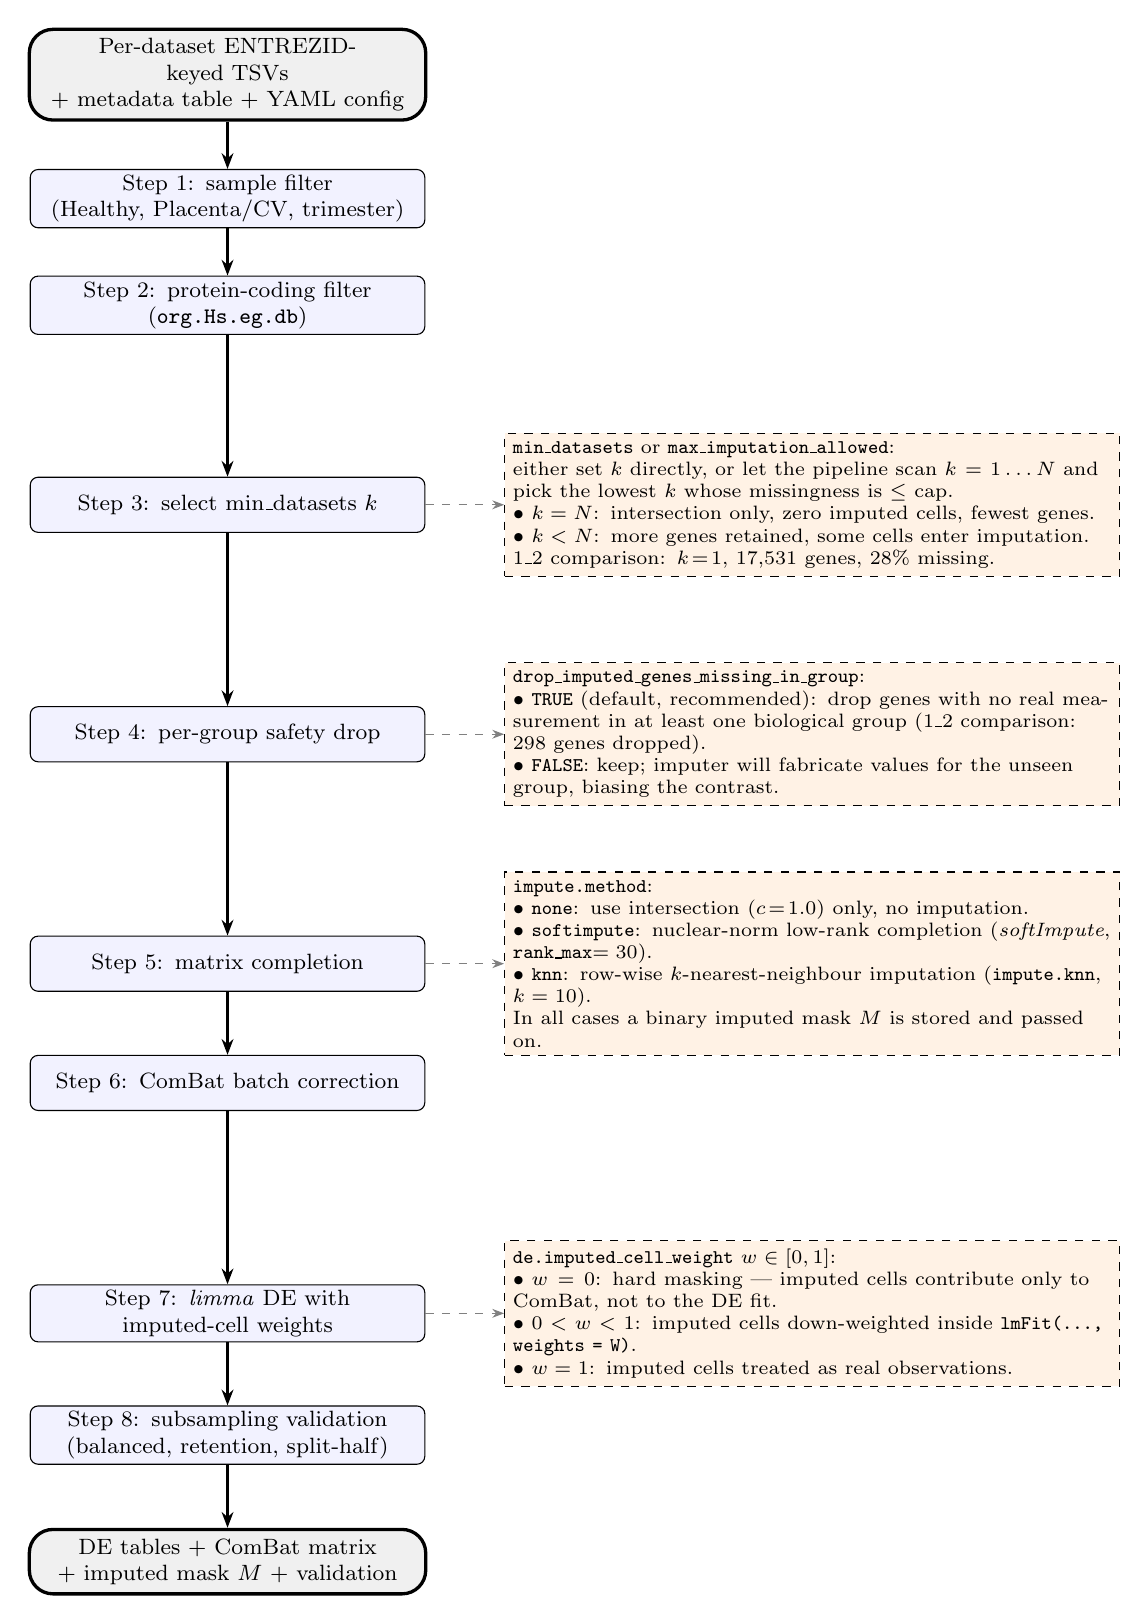
\begin{tikzpicture}[
  node distance=6mm and 10mm,
  every node/.style={font=\footnotesize},
  flowstep/.style={rectangle, rounded corners=1mm, draw, fill=blue!5,
    align=center, minimum height=7mm, inner xsep=3pt, inner ysep=2pt,
    text width=48mm},
  param/.style={rectangle, draw, dashed, fill=orange!10, align=left,
    inner sep=3pt, text width=76mm, font=\scriptsize},
  term/.style={rectangle, rounded corners=3mm, draw, very thick,
    fill=gray!12, align=center, minimum height=7mm, text width=48mm},
  arr/.style={-{Stealth[length=2mm]}, thick},
  darr/.style={-{Stealth[length=1.5mm]}, dashed, gray}
]

\node[term] (in) {Per-dataset ENTREZID-keyed TSVs\\
  + metadata table + YAML config};
\node[flowstep, below=6mm of in] (s1) {Step~1: sample filter\\
  (Healthy, Placenta/CV, trimester)};
\node[flowstep, below=6mm of s1] (s2) {Step~2: protein-coding filter\\
  (\texttt{org.Hs.eg.db})};
\node[flowstep, below=18mm of s2] (s3) {Step~3: select min\_datasets $k$};
\node[flowstep, below=22mm of s3] (s4) {Step~4: per-group safety drop};
\node[flowstep, below=22mm of s4] (s5) {Step~5: matrix completion};
\node[flowstep, below=8mm of s5] (s6) {Step~6: ComBat batch correction};
\node[flowstep, below=22mm of s6] (s7) {Step~7: \textit{limma} DE with
  imputed-cell weights};
\node[flowstep, below=8mm of s7] (s8) {Step~8: subsampling validation\\
  (balanced, retention, split-half)};
\node[term, below=8mm of s8] (out) {DE tables + ComBat matrix\\
  + imputed mask $M$ + validation};

\draw[arr] (in) -- (s1);
\draw[arr] (s1) -- (s2);
\draw[arr] (s2) -- (s3);
\draw[arr] (s3) -- (s4);
\draw[arr] (s4) -- (s5);
\draw[arr] (s5) -- (s6);
\draw[arr] (s6) -- (s7);
\draw[arr] (s7) -- (s8);
\draw[arr] (s8) -- (out);

\node[param, right=of s3] (p3) {%
  \textbf{\texttt{min\_datasets}} or
  \textbf{\texttt{max\_imputation\_allowed}}:\\
  either set $k$ directly, or let the pipeline scan
  $k = 1 \ldots N$ and pick the lowest $k$ whose
  missingness is $\le$ cap.\\
  $\bullet$ $k = N$: intersection only, zero imputed cells,
  fewest genes.\\
  $\bullet$ $k < N$: more genes retained, some cells enter
  imputation.\\
  1\_2 comparison: $k\!=\!1$, 17{,}531 genes, 28\% missing.};
\draw[darr] (s3.east) -- (p3.west);

\node[param, right=of s4] (p4) {%
  \textbf{\texttt{drop\_imputed\_genes\_missing\_in\_group}}:\\
  $\bullet$ \texttt{TRUE} (default, recommended): drop genes
  with no real measurement in at least one biological group
  (1\_2 comparison: 298 genes dropped).\\
  $\bullet$ \texttt{FALSE}: keep; imputer will fabricate values
  for the unseen group, biasing the contrast.};
\draw[darr] (s4.east) -- (p4.west);

\node[param, right=of s5] (p5) {%
  \textbf{\texttt{impute.method}}:\\
  $\bullet$ \texttt{none}: use intersection ($c\!=\!1.0$) only,
  no imputation.\\
  $\bullet$ \texttt{softimpute}: nuclear-norm low-rank completion
  (\textit{softImpute}, \texttt{rank\_max}$=30$).\\
  $\bullet$ \texttt{knn}: row-wise $k$-nearest-neighbour
  imputation (\texttt{impute.knn}, $k=10$).\\
  In all cases a binary imputed mask $M$ is stored and passed
  on.};
\draw[darr] (s5.east) -- (p5.west);

\node[param, right=of s7] (p7) {%
  \textbf{\texttt{de.imputed\_cell\_weight}} $w \in [0,1]$:\\
  $\bullet$ $w = 0$: hard masking --- imputed cells contribute
  only to ComBat, not to the DE fit.\\
  $\bullet$ $0 < w < 1$: imputed cells down-weighted inside
  \texttt{lmFit(\ldots, weights = W)}.\\
  $\bullet$ $w = 1$: imputed cells treated as real observations.};
\draw[darr] (s7.east) -- (p7.west);

\end{tikzpicture}
\caption{Direct-merge pipeline overview with parameter-dependent
  branching. Solid arrows show the deterministic flow from
  inputs (top) through the seven method steps to outputs
  (bottom); dashed callouts list the configurable options at
  each branching step and their downstream consequences. The
  configuration used for the results in
  Tables~\ref{tab:recovery}--\ref{tab:de} is:
  \texttt{max\_imputation\_allowed} $=1.0$,
  \texttt{drop\_imputed\_genes\_missing\_in\_group} $=$
  \texttt{TRUE},
  \texttt{impute.method} $=$ \texttt{softimpute},
  ComBat-ref (reference batch: GSE100051), and
  \texttt{de.imputed\_cell\_weight} $w = 0$ (hard masking).}
\label{fig:pipeline}
\end{figure}

\subsection{Input harmonisation and sample filtering}

The pipeline (\texttt{run\_phase2b.R}) consumes a YAML
configuration file that specifies (a) the directory containing
ENTREZID-keyed expression TSVs, (b) the metadata table with
sample-level annotations, (c) the biological contrast (baseline vs.
contrast group) and any covariates (e.g.~\textit{Fetus.Sex}),
and (d) tuning parameters for downstream steps. Each expression
file is read and filtered to samples matching a \texttt{Diagnosis}
$=$ ``Healthy'', \texttt{Biological.Specimen} $\in$
\{``Placenta'', ``Chorionic villi''\}, and the two
gestational-age categories of interest.

\subsection{Protein-coding gene filter}

This filter is applied \emph{before} matrix
completion so that matrix factorisation does not attempt to
model non-coding RNAs, pseudogenes, and retired identifiers.
Per-dataset expression matrices are intersected with the set of
ENTREZIDs for which
\texttt{org.Hs.eg.db::GENETYPE == "protein-coding"}.
An audit against the current NCBI \texttt{Homo\_sapiens.gene\_info}
release confirmed that no protein-coding genes were lost by
using the installed Bioconductor snapshot.

\subsection{Minimum dataset-presence selection}

The user specifies the minimum number of datasets $k$ in which
a gene must be present for inclusion in the merged matrix. Two
mutually exclusive configuration modes are available:

\begin{enumerate}
  \item \textbf{Fixed \texttt{min\_datasets}}: the value of $k$
    is set directly in the configuration file.
  \item \textbf{Auto-selection via
    \texttt{max\_imputation\_allowed}}: the pipeline scans
    $k = 1, 2, \ldots, N$ and selects the lowest $k$ whose
    post-drop missing fraction does not exceed the cap.
\end{enumerate}

\subsection{Per-group imputation safety check}
\label{sec:coverage}

For every gene that requires imputation in at least one dataset,
the pipeline counts the number of \emph{non-imputed} samples
available in each of the two biological groups. Genes that lack
any real measurement in one of the two groups are dropped
(configurable via
\texttt{drop\_imputed\_genes\_\allowbreak missing\_in\_group}), because
matrix completion under a sparse row with no group-specific
evidence would otherwise synthesise an arbitrary value under the
unseen condition and bias the contrast.

\subsection{Matrix completion}

Two imputation methods are available:
\begin{enumerate}
  \item \textit{softImpute} \citep{Mazumder2010,Hastie2015}:
    low-rank matrix completion regularised by the nuclear norm
    (the sum of the matrix's singular values, which penalises
    solutions that use more latent factors than necessary). The
    algorithm iteratively decomposes the observed portion of the
    matrix into a small number of latent factors and reconstructs
    the missing entries from those factors, with a warm-start
    $\lambda$ path and column centring/scaling by
    \texttt{biScale}; default \texttt{rank\_max} $= 30$,
    $\lambda$ auto-selected along an 8-point path. Low-rank
    matrix completion of this family has been used extensively
    for transcriptomics imputation, primarily in single-cell
    RNA-seq (e.g.~McImpute, \citealp{Mongia2019}), though it is
    rarely applied to bulk microarray meta-analysis.
  \item \textit{impute::impute.knn} \citep{Troyanskaya2001}:
    $k$-nearest-neighbour row imputation with $k = 10$. KNN
    imputation is the de-facto standard for missing-value recovery
    in microarray studies and has been evaluated in numerous
    comparative reviews
    \citep{Aittokallio2010,Liew2011}.
\end{enumerate}
A binary \texttt{imputed\_mask} is stored alongside the completed
matrix and carried through all subsequent steps.

\subsection{ComBat batch correction}

The completed matrix is batch-corrected with
\texttt{sva::ComBat} using a model matrix of
$\sim\!\text{bio\_group}+\text{fetus\_sex}$, where
\texttt{bio\_group} is the two-level contrast. We use the
reference-batch variant of ComBat (\texttt{ref.batch}
parameter), which adjusts all other batches toward the
reference batch rather than toward the grand mean. GSE100051
was chosen as reference because it is the largest dataset
(49 of 117 samples) and spans both comparison groups (42
first-trimester, 7 second-trimester). Parametric empirical
Bayes priors are enabled.

\subsection{Differential expression with imputed-cell
  weighting}

Differential expression is computed with \texttt{limma::lmFit}
followed by \texttt{eBayes} and \texttt{topTable}. A per-cell
weight matrix $W$ is constructed from the imputed mask:
$W_{ij} = 1$ for real observations and
$W_{ij} = w$ for imputed ones, with
$w \in [0, 1]$ controlled by \texttt{de.imputed\_cell\_weight}.
Setting $w = 0$ realises hard masking (imputed cells contribute
only to batch correction, not to the DE fit), while $w = 1$
treats imputed cells as real. We use $w = 0$ (hard masking) as
the default: imputed values stabilise the batch-effect
estimation in ComBat by providing a complete matrix, but are
excluded from the expression contrast so that differential
expression calls are driven entirely by real measurements.
When a dataset contains technical replicates --- multiple
arrays hybridised from the same biological sample --- treating
them as independent observations would inflate the effective
sample size and produce anti-conservative $p$-values. The
pipeline handles this via \texttt{limma}'s mixed-model
machinery: a \texttt{technical\_replicate\_block} column in the
metadata table assigns each array to its biological sample.
Samples without replicates receive singleton pseudo-block
identifiers. \texttt{duplicateCorrelation()} estimates the
consensus intra-block correlation across all genes, and the
resulting correlation and block vector are passed to
\texttt{lmFit(\ldots, block = block\_vec, correlation =
corfit\$consensus.correlation)}, so that the linear model
accounts for the within-sample covariance. This mechanism
operates jointly with the imputed-cell weight matrix $W$ when
both are present. In the 1\_2 comparison reported here none of
the six datasets contain technical replicates, so this path
is not exercised; it becomes active in other contrasts that
include GSE55439 (6 biological samples profiled in 3--6
technical replicates each, 24 arrays total).

Thresholds for the significant-gene list are
$\text{adj.P.Val} < 0.05$ and $|\text{logFC}| > 1$.
Differential expression is computed with \textit{limma}'s
empirical Bayes moderation \citep{Smyth2004, Ritchie2015}.

\subsection{Software and data resources}

All quantitative steps are parameterised from a single YAML
configuration file and logged to a timestamped
\texttt{phase2b\_log\_<datetime>.txt}. Each run writes the
imputation validation table, the gene recovery comparison, the
per-group coverage audit, the method comparison table, the
per-method completed expression matrices, the per-method ComBat
output matrices, and the per-method differential expression
tables (both full and filtered).

The principal software dependencies are listed in
Table~\ref{tab:resources}.

\begin{table}[h]
\centering
\footnotesize
\begin{tabularx}{\textwidth}{@{}l l X l@{}}
\toprule
\textbf{Resource} & \textbf{Source} & \textbf{Identifier} & \textbf{Notes} \\
\midrule
\multicolumn{4}{l}{\emph{Deposited data}} \\
Raw and normalised expression data & NCBI GEO & GSE100051, GSE122214, GSE28551, GSE37901, GSE93520, GSE9984 & Healthy placenta / chorionic villi \\
Human gene annotations & Bioconductor & \texttt{org.Hs.eg.db} 3.21.0 & Protein-coding \\
\addlinespace
\multicolumn{4}{l}{\emph{Software and algorithms}} \\
R (statistical environment) & R Core Team & R $\ge$ 4.3 & CRAN \\
\texttt{sva::ComBat} & Leek et al. & Bioconductor & Batch correction \\
\texttt{limma} & Ritchie et al. & Bioconductor & Diff.\ expression \\
\texttt{softImpute} & Hastie et al. & CRAN & Matrix completion \\
\texttt{impute::impute.knn} & Troyanskaya et al. & Bioconductor & KNN imputation \\
\texttt{AnnotationDbi} & Bioconductor & --- & Gene metadata \\
Pipeline source code & This study & [to be deposited] & Reproducible \\
\bottomrule
\end{tabularx}
\caption{Software and data resources used in this study. GEO
  accessions list the six placental microarray datasets; gene
  annotations were used for protein-coding filtering. The
  principal R packages for batch correction, differential
  expression, and matrix-completion imputation are listed.}
\label{tab:resources}
\end{table}

%% =========================================================================
%% Declarations (BMC Bioinformatics required sections)
%% =========================================================================

\section*{Declarations}

\subsection*{Ethics approval and consent to participate}
Not applicable. This study uses only publicly available data
from the NCBI Gene Expression Omnibus (GEO). Ethics approval
for each original study was obtained by the respective
depositing investigators as described in the source publications.

\subsection*{Consent for publication}
Not applicable.

\subsection*{Availability of data and materials}
All expression datasets analysed in this study are available
from the NCBI Gene Expression Omnibus under accession numbers
GSE100051, GSE122214, GSE28551, GSE37901, GSE93520,
and GSE9984. The pipeline source code and YAML configurations
will be deposited in a public repository prior to publication.
%% TODO: add GitHub URL and Zenodo DOI once deposited.

\subsection*{Competing interests}
The authors declare that they have no competing interests.

\subsection*{Funding}
%% TODO: add funding information.

\subsection*{Authors' contributions}
%% TODO: add author contributions.

%% =========================================================================
\section*{Acknowledgements}
%% =========================================================================
%% TODO: add acknowledgements.

%% =========================================================================
%% References
%% =========================================================================
\begin{thebibliography}{99}

\bibitem[Bianco et al.(2016)]{Bianco2016}
Bianco, K., Bhatt, S., Engel, N., Glessner, J. T., \&
Bhatt, S. S. (2016). Placental transcriptomes in the common
aneuploidies reveal critical regions on the trisomic
chromosomes. \emph{Prenatal Diagnosis}, 36(8), 760--769.
\doi{10.1002/pd.4862}

\bibitem[Aittokallio(2010)]{Aittokallio2010}
Aittokallio, T. (2010). Dealing with missing values in
large-scale studies: microarray data imputation and beyond.
\emph{Briefings in Bioinformatics}, 11(2), 253--264.
\url{https://doi.org/10.1093/bib/bbp059}

\bibitem[Hastie et al.(2015)]{Hastie2015}
Hastie, T., Mazumder, R., Lee, J. D., \& Zadeh, R. (2015).
Matrix completion and low-rank SVD via fast alternating least
squares. \emph{Journal of Machine Learning Research}, 16,
3367--3402.

\bibitem[Hu et al.(2006)]{Hu2006}
Hu, J., Li, H., Waterman, M. S., \& Zhou, X. J. (2006).
Integrative missing value estimation for microarray data.
\emph{BMC Bioinformatics}, 7, 449.
\url{https://doi.org/10.1186/1471-2105-7-449}

\bibitem[Johnson et al.(2007)]{Johnson2007}
Johnson, W. E., Li, C., \& Rabinovic, A. (2007). Adjusting batch
effects in microarray expression data using empirical Bayes
methods. \emph{Biostatistics}, 8(1), 118--127.

\bibitem[Lin(1989)]{Lin1989}
Lin, L. I-K. (1989). A concordance correlation coefficient to
evaluate reproducibility. \emph{Biometrics}, 45(1), 255--268.
\doi{10.2307/2532051}

\bibitem[Leek et al.(2012)]{Leek2012}
Leek, J. T., Johnson, W. E., Parker, H. S., Jaffe, A. E., \&
Storey, J. D. (2012). The sva package for removing batch effects
and other unwanted variation in high-throughput experiments.
\emph{Bioinformatics}, 28(6), 882--883.

\bibitem[Li et al.(2019)]{Li2019}
Li, Y., Wang, L., Zhou, J., \& Ye, J. (2019). Multi-task
learning based survival analysis for multi-source block-wise
missing data. \emph{Neurocomputing}, 364, 95--107.
\url{https://doi.org/10.1016/j.neucom.2019.07.010}

\bibitem[Liew et al.(2011)]{Liew2011}
Liew, A. W.-C., Law, N.-F., \& Yan, H. (2011). Missing value
imputation for gene expression data: computational techniques to
recover missing data from available information.
\emph{Briefings in Bioinformatics}, 12(5), 498--513.
\url{https://doi.org/10.1093/bib/bbq080}

\bibitem[Lykhenko et al.(2021a)]{Lykhenko2021a}
Lykhenko, O., Frolova, A., \& Obolenskaya, M. (2021).
Consecutive integration of available microarray data for
analysis of differential gene expression in human placenta.
\emph{Biotechnologia Acta}, 14(1), 38--45.
\url{https://doi.org/10.15407/biotech14.01.38}

\bibitem[Lykhenko et al.(2021b)]{Lykhenko2021b}
Lykhenko, O., Frolova, A., \& Obolenskaya, M. (2021). Changes
in the human placental transcriptome during the physiological
course of pregnancy. \emph{Biopolymers and Cell}, 37(1),
73--82. \url{https://doi.org/10.7124/bc.000A4D}

\bibitem[Mikheev et al.(2008)]{Mikheev2008}
Mikheev, A.M., Nabekura, T., Kaddoumi, A., Bammler, T.K.,
Govindarajan, R., Hebert, M.F., \& Unadkat, J.D. (2008).
Profiling gene expression in human placentae of different
gestational ages: an OPRU Network and UW SCOR Study.
\emph{Reproductive Sciences}, 15(9), 866--877.
\doi{10.1177/1933719108322425}

\bibitem[Mazumder et al.(2010)]{Mazumder2010}
Mazumder, R., Hastie, T., \& Tibshirani, R. (2010). Spectral
regularization algorithms for learning large incomplete matrices.
\emph{Journal of Machine Learning Research}, 11, 2287--2322.

\bibitem[Mongia et al.(2019)]{Mongia2019}
Mongia, A., Sengupta, D., \& Majumdar, A. (2019). McImpute:
Matrix completion based imputation for single cell RNA-seq data.
\emph{Frontiers in Genetics}, 10, 9.
\url{https://doi.org/10.3389/fgene.2019.00009}

\bibitem[Rull et al.(2013)]{Rull2013}
Rull, K., Tomberg, K., K\~{o}ks, S., M\"{a}nnik, J.,
M\"{o}ls, M., Sirotkina, M., V\"{a}rv, S., \& Laan, M. (2013).
Increased placental expression and maternal serum levels of
apoptosis-inducing \emph{TRAIL} in recurrent miscarriage.
\emph{Placenta}, 34(2), 141--148.
\doi{10.1016/j.placenta.2012.11.032}

\bibitem[Ritchie et al.(2015)]{Ritchie2015}
Ritchie, M. E., Phipson, B., Wu, D., Hu, Y., Law, C. W., Shi, W.,
\& Smyth, G. K. (2015). limma powers differential expression
analyses for RNA-sequencing and microarray studies.
\emph{Nucleic Acids Research}, 43(7), e47.

\bibitem[Sitras et al.(2012)]{Sitras2012}
Sitras, V., Fenton, C., Paulssen, R., V\aa{}rtun, \AA., \&
Acharya, G. (2012). Differences in gene expression between first
and third trimester human placenta: a microarray study.
\emph{PLoS ONE}, 7(3), e33294.
\doi{10.1371/journal.pone.0033294}

\bibitem[Soncin et al.(2018)]{Soncin2018}
Soncin, F., Khater, M., To, C., Pizzo, D., Farah, O.,
Wakeland, A., Arul Nambi Rajan, K., Nelson, K.K., Chang, C.-W.,
Moretto-Zita, M., Natale, D.R., Laurent, L.C., \& Parast, M.M.
(2018). Comparative analysis of mouse and human placentae across
gestation reveals species-specific regulators of placental
development. \emph{Development}, 145(2), dev156273.
\doi{10.1242/dev.156273}

\bibitem[Smyth(2004)]{Smyth2004}
Smyth, G. K. (2004). Linear models and empirical Bayes methods
for assessing differential expression in microarray experiments.
\emph{Statistical Applications in Genetics and Molecular
Biology}, 3(1), Article 3.

\bibitem[Tuikkala et al.(2006)]{Tuikkala2006}
Tuikkala, J., Elo, L., Nevalainen, O. S., \& Aittokallio, T.
(2006). Improving missing value estimation in microarray data
with gene ontology. \emph{Bioinformatics}, 22(5), 566--572.
\url{https://doi.org/10.1093/bioinformatics/btk019}

\bibitem[Tuikkala et al.(2008)]{Tuikkala2008}
Tuikkala, J., Elo, L. L., Nevalainen, O. S., \& Aittokallio, T.
(2008). Missing value imputation for microarray gene expression
data using histone acetylation information.
\emph{BMC Bioinformatics}, 9, 252.
\url{https://doi.org/10.1186/1471-2105-9-252}

\bibitem[Uusk\"{u}la et al.(2012)]{Uuskula2012}
Uusk\"{u}la, L., M\"{a}nnik, J., Rull, K., Minajeva, A.,
K\~{o}ks, S., Vaas, P., Teesalu, P., Reimand, J., \& Laan, M.
(2012). Mid-gestational gene expression profile in placenta and
link to pregnancy complications. \emph{PLoS ONE}, 7(11), e49248.
\doi{10.1371/journal.pone.0049248}

\bibitem[Troyanskaya et al.(2001)]{Troyanskaya2001}
Troyanskaya, O., Cantor, M., Sherlock, G., Brown, P., Hastie, T.,
Tibshirani, R., Botstein, D., \& Altman, R. B. (2001). Missing
value estimation methods for DNA microarrays.
\emph{Bioinformatics}, 17(6), 520--525.

\bibitem[Walsh et al.(2015)]{Walsh2015}
Walsh, C. J., Hu, P., Batt, J., \& Dos Santos, C. C. (2015).
Microarray meta-analysis and cross-platform normalization:
integrative genomics for robust biomarker discovery.
\emph{Microarrays}, 4(3), 389--406.
\url{https://doi.org/10.3390/microarrays4030389}

\bibitem[Zhang et al.(2017)]{Zhang2017}
Zhang, B., Feng, L., Guo, H., Li, H., Yang, R., Wang, Y.,
Zhang, K., Yu, X., \& Cheng, S. (2017). Villi-specific gene
expression reveals novel prognostic biomarkers in multiple human
cancers. \emph{Journal of Cancer}, 8(14), 2793--2801.
\doi{10.7150/jca.19787}

\bibitem[Zhao et al.(2019)]{Zhao2019}
Zhao, L., Zheng, X., Liu, J., Zheng, R., Yang, R., Wang, Y.,
\& Sun, L. (2019). The placental transcriptome of the
first-trimester placenta is affected by in vitro fertilization
and embryo transfer. \emph{Reproductive Biology and
Endocrinology}, 17, 50.
\doi{10.1186/s12958-019-0494-7}

\bibitem[Zheng and Tang(2024)]{Zheng2024}
Zheng, R., \& Tang, M. (2024). Chain-linked multiple matrix
integration via embedding alignment. \emph{arXiv preprint}
arXiv:2412.02791.
\url{https://arxiv.org/abs/2412.02791}

\bibitem[Zhou et al.(2017)]{Zhou2017}
Zhou, W., Han, L., \& Altman, R. B. (2017). Imputing gene
expression to maximize platform compatibility.
\emph{Bioinformatics}, 33(4), 522--528.
\url{https://doi.org/10.1093/bioinformatics/btw664}

\bibitem[Zhou et al.(2021)]{Zhou2021}
Zhou, D., Cai, T., \& Lu, J. (2021). Multi-source learning via
completion of block-wise overlapping noisy matrices.
\emph{arXiv preprint} arXiv:2105.10360.
\url{https://arxiv.org/abs/2105.10360}

\end{thebibliography}

%% =========================================================================
%% Additional files (supplements)
%% =========================================================================

\section*{Additional files}

\subsection*{Additional file 1 --- Alternatives and supplements to ComBat}
Review of batch correction alternatives (SVA, RUV, reference-batch ComBat,
MNN/Harmony, HarmonizR, batch-sensitized imputation, effect-size
meta-analysis) for integrating microarray studies with non-overlapping
biological groups, with recommendations for the placenta pipeline.
(PDF, supplement1.pdf)

\subsection*{Additional file 2 --- RUV negative control gene selection}
Strategies for assembling negative control gene lists for RUV in
placental transcriptome studies across gestational ages, including
empirical validation against pipeline results and a comparative
benchmark of RUV versus ComBat.
(PDF, supplement2.pdf)

\end{document}
